% made by: KorG
% vim: ft=tex et :
\documentclass[oneside]{book}

\usepackage[T1,T2A]{fontenc}       % fonts
\usepackage[utf8]{inputenc}     % UTF-8
\usepackage[english,russian]{babel}     % russian
\usepackage{cmap}               % russian search in pdf
\usepackage{pscyr}		        % PSCyr
\usepackage[14pt]{extsizes}     % for compatibility
\usepackage{float}		        % essential for [H]

\usepackage{indentfirst}        % first string indention

\usepackage{graphicx}           % graphics
\usepackage{ltxtable}           % tables

\usepackage{amsmath}            % math
\usepackage{nccmath}            % math medium sizes
\usepackage{amsfonts}           % math fonts
\usepackage{amssymb}            % math symb
\usepackage[a4paper, left=2cm, right=2cm, top=2cm,
        bottom=3cm]{geometry}   % pagesize

\usepackage{color}
\usepackage{xcolor}
\definecolor{light-gray}{gray}{0.9}

\usepackage{titlesec}
\usepackage{float}
\usepackage{multirow}
\usepackage{tabularx}
\usepackage{placeins}
\usepackage{totcount}
\usepackage[hidelinks,pdftex]{hyperref}
\usepackage[numbers,sort&compress]{natbib}
\usepackage{caption}
\usepackage{subcaption}
\frenchspacing
\setcounter{page}{1}
\bibliographystyle{utf8gost705u}
\makeatletter % [1] -> 1.
\renewcommand\@biblabel[1]{#1.}
\makeatother
\addto\captionsrussian{\def\refname{Библиографический список}}
\regtotcounter{page}
\regtotcounter{figure}
\regtotcounter{table}
\captionsetup{justification=centering,labelsep=period}
\captionsetup[table]{aboveskip=0pt,belowskip=0pt}

\usepackage{soul}               % \so{} & \ul{} - source and underline
\usepackage{soulutf8}           % UTF-8 for soul
\usepackage{verbatim}           % \verb{} and verbatim environment
\usepackage{listings}           % source code `bl
\lstset{
   escapeinside={\#@}{@},
        extendedchars=\true,
        numbers=left,
        inputencoding=utf8,
        keepspaces=true,
        basicstyle=\footnotesize\ttfamily,
        backgroundcolor=\color{light-gray},
        tabsize=3,
        breaklines=true,
        postbreak=\raisebox{0ex}[0ex][0ex]{\ensuremath{\color{red}\hookrightarrow\space}}
     }

\usepackage{fancyhdr}
\pagestyle{fancy}
\fancyhf{}                      % clear header and footer
\fancyfoot[C]{\thepage}         % page number
\renewcommand{\headrulewidth}{0pt}      % remove that line

\linespread{1.4}                % line interval ~1.5
\renewcommand{\rmdefault}{ftm}

\newcommand\header[3]{          % `H {sub}{*}{TITLE}
   \def \a {#1}
   \def \b {sub}
   \ifx\a\b
   \subsection#2{#3}
   \else
   \section#2{#3}
   \fi
   \ifx x#2x
   \else
   \addcontentsline{toc}{#1section}{#3}
   \fi
}

% ------------------------------
% Table of contents

\setcounter{secnumdepth}{4}
\usepackage{mathtext}
\renewcommand*{\familydefault}{\sfdefault} % clear font defaults
\usepackage{microtype}
\sloppy

% ------------------------------
% Page geometry & text spacing

\usepackage{parskip}
\setlength{\parindent}{0em}
\setlength{\parskip}{1em}

%% \usepackage{atbegshi} % http://ctan.org/pkg/atbegshi
%% \AtBeginDocument{\AtBeginShipoutNext{\AtBeginShipoutDiscard}}

\let\OLDitemize\itemize % itemize spacing
\renewcommand\itemize{\OLDitemize\addtolength{\itemsep}{-5pt}}

   \renewcommand{\arraystretch}{1.5}

   % ------------------------------
   % Code listings

\definecolor{mGreen}{rgb}{0,0.6,0}
\definecolor{mGray}{rgb}{0.5,0.5,0.5}
\definecolor{mPurple}{rgb}{0.58,0,0.82}
\definecolor{backgroundColour}{rgb}{0.95,0.96,0.97}


% C language codestyle
\lstdefinestyle{CStyle}{
   backgroundcolor=\color{backgroundColour},   
    commentstyle=\color{mGreen},
    keywordstyle=\color{blue},
    numberstyle=\tiny\color{mGray},
    stringstyle=\color{mPurple},
    basicstyle=\footnotesize,
    breakatwhitespace=false,         
    breaklines=true,                 
    captionpos=b,                    
    keepspaces=true,                 
    numbers=left,                    
    numbersep=5pt,                  
    showspaces=false,                
    showstringspaces=false,
    showtabs=false,                  
    tabsize=2,
    postbreak=\%\space,
    %belowskip=-1,
    language=C
 }

 % sh language codestyle
\lstdefinestyle{shStyle} {
   backgroundcolor=\color{backgroundColour},   
    commentstyle=\color{mGreen},
    keywordstyle=\color{magenta},
    numberstyle=\tiny\color{mGray},
    stringstyle=\color{mPurple},
    basicstyle=\footnotesize,
    breakatwhitespace=false,         
    breaklines=true,                 
    captionpos=b,                    
    keepspaces=true,                 
    numbers=left,                    
    numbersep=5pt,                  
    showspaces=false,                
    showstringspaces=false,
    showtabs=false,                  
    tabsize=2,
    postbreak=\%\space,
    morecomment=[s][\color{red}]{\ -}{\ },
    otherkeywords={$,@,>,<,\#,!,ELIF,IF,THEN,ELSE,FI,ESAC,CASE,WHILE,DO,UNTIL,FOR,echo,man,chmod},
    language=sh
 }
 %$$

 % listings titles style
\newenvironment{funci}[1]{{{\textbf{#1}}}}{}

% for C language code
\lstnewenvironment{CCode}[1]{
   \lstset{style=cStyle}
   \funci{#1}~}{
}

% for sh code
\lstnewenvironment{shCode}[1]{
   \lstset{style=shStyle}
   \funci{#1}~}{
}

% ------------------------------
% Special commands an environments


% for spaced environvent (example^ prompt string section)
\newenvironment{myenv}[2]{
   \renewcommand{\tabcolsep}{0cm}
   \begin{tabular}{p{0.15\linewidth}p{0.85\linewidth}}
      \textbf{#1} & #2
   \end{tabular}\\[0.5em]
   }{
      }

\usepackage{xpatch}
\makeatletter
\xpatchcmd{\@thm}{\thm@headpunct{.}}{\thm@headpunct{ --- \\}}{}{}
\makeatother

% for definitions
\newenvironment{defi}[1]{
   \textbf{#1} ---
      \\[0.3em]
      \begin{tabular}{p{0.5\linewidth}p{0.9\linewidth}}
         & 
         }
         {
      \end{tabular}
      }

      % for important addings	
\newenvironment{important}{\textbf{Важно: }{}}

\newenvironment{boxy}{
   \renewcommand{\arraystretch}{1.8}
   \begin{tabular}{|p{1\linewidth}|}
      \hline
      }
      {
         \\ \hline
   \end{tabular}
   }

\begin{document}

\cleardoublepage\clearpage


\begin{titlepage}
	% \centering	
	\Large ПРОЕКТ УЧЕБНОГО ПОСОБИЯ
	
	\vspace {4cm}
	
	\Huge\textbf{{\fontsize{30}{30}\selectfont 
	ОСНОВЫ СИСТЕМНОГО
	\\
	ПРОГРАММИРОВАНИЯ}}
	
	\vspace{0.5cm}
	{\large Операционная система UNIX, интерпретатор shell, язык C \par}
	


	\vfill
	{\large НИУ ИТМО, 2018}
	
\end{titlepage}

\clearpage

\tableofcontents

\clearpage 
\addcontentsline{toc}{chapter}{Благодарности}
\chapter*{Благодарности}
Выражается особая благодарность людям, внесшим большой вклад в составление первой редакции  учебного пособия:

\begin{itemize}

	\item Александре Горской (2015 г. поступления) --- выборка, редактура и верстка 		материалов первой версии пособия;
	
	
\end{itemize}
 

% ------------------------------
% Часть: Основы системного программирования

\clearpage \part{Системное программное обеспечение}
%Многие из вас, уже успели поработать с shell и успели понять, что такое ввод команд и реакция системы на это. 

Сразу обозначим одну вещь --- если мы хотим программировать нужно использовать инструменты для программирования, а не shell. Shell, это командный интерпретатор, инструмент, который позволяет автоматизировать запуск команд, а не писать сложные алгоритмы. Чаще всего shell скрипт не должен быть интерактивным, а должен автоматизировать выполнение каких-то команд. При работе с командным интерпретатором нам не должно быть интересно постоянно инструктировать скрипт о том, что ему делать. 

В этом разделе мы рассмотрим базовые принципы взаимодействия с операционной системой UNIX посредством командного интерпретатора.

   \chapter{Операционная система}

      \section{Роль операционной системы}
      Операционная система предоставляет пользователю следующую функциональность:

\textbf{Многозадачность}

Позволяет одновременно выполнять несколько программ, изолируя их в разных адресных пространствах.

\textbf{Виртуализация памяти}

Операционная система абстрагирует программиста от физического адресного пространства, позволяет использовать больше адресного пространства, чем доступно оперативной памяти, а также изолирует программы, размещая их по непересекающимся адресам.

\textbf{Управление устройствами}

Система позволяет нам абстрагироваться от взаимодействия с устройствами, беря эту задачу на себя.

В самом деле, было бы сложно каждый раз самим думать о том как, например, спозиционировать читающую головку на жестком диске или как вывести что-то на принтер.

\textbf{Обработка прерываний}

Операционная система реагирует на события, которые являются внешними по отношению к процессу (например, запрос на ввод-вывод). Такие события называются прерываниями.

\textbf{Расширение набора операций, доступных программам}

Операционная система расширяет набор команд, доступных программам. На уровне операционной системы появляются системные вызовы --- обращения к функциям, которые реализованы в ядре операционной системы. 

      \section{Типовая ОС UNIX}
      Архитектура операционной системы UNIX является многоуровневой:

На самом внутреннем уровне распологается ядро. Функции ядра доступны через интерфейс системных вызовов. На среднем уровене находятся системные утилиты, демоны, драйверы, протоколы. На внешнем уровне --- прикладные программы пользователя.


      \section{Ядро типовой ОС UNIX}
      Ядро --- это центральная часть операционной системы. Ядро загружается и работает в младшей части адресного пространства оперативной памяти, таким образом, чтобы виртуальные и физические адреса соответствовали друг другу. 

Ядро является своего рода большим диспетчером, обычной программой, которая работает на процессоре. Системные вызовы --- механизм обращения к функциям ядра. В адресном пространстве ядра располагаются обработчики событий, сигналов, прерываний, исключений. 

При переходе из режима задачи в режим ядра система разрешает доступ к этим адресам, а при обратном переходе --- запрещает. 

         \subsection{Подсистемы ядра}
         Ядро операционной системы UNIX состоит из следующих подсистем:

\begin{itemize}
	\item \textbf{Файловая подсистема}

		Эта подсистема определяет унифицированный интерфейс доступа к файлам. Отвечает за такие процессы, как создание, удаление, чтение и запись файлов. Также файловая подсистема обеспечивает контроль прав доступа к файлам.

	\item \textbf{Подсистема управления процессами и памятью}

		Подсистема управления процессами занимается планированием процессорного времени, инициализацией и завершением процессов. Отвечает за синхронизацию , а также за распредление системных ресурсов между процессами.

	\newpage
	\item \textbf{Подсистема ввода-вывода}

		Данная подсистема берет на себя взаимодействие с драйверами устройств и обеспечивает буферизацию данных.
\end{itemize}


         \subsection{Исключения, прерывания, системные вызовы}

            \subsubsection{Исключения}
            Если при выполнении программы процесс пытается выполнить некорректную операцию, например, деление на ноль или доступ к участку памяти, который ему недоступен, то генерируется исключение. Исключение переключает процессор в режим ядра и вызывает обработчик исключений.

Обработчик исключений, в свою очередь, должен определить, может ли процесс восстановиться после ошибки. Если да, он выполняет действия по восстановлению и переводит процесс обратно в режим задачи, не сообщая о произошедшей ошибке.

Иначе выполняются действия по аварийному завершению работы процесса.

            \subsubsection{Прерывания}
            \begin{defi}{Прерывание}
	это приостановка выполнения программы по специальному сигналу.
\end{defi}

Механизм прерываний нужен для оповещения системы об асинхронных событиях, таких, как нажатие клавиши на клавиатуре.

При выработке прерываний выполняется переход в режим ядра и поиск обработчика прерывания в IDT --- Interrupt Descriptor Table. После исполнения обработчика прерываний выполняется обратный переход --- в режим задачи.

Разница между исключениями и прерываниями состоит в том, что исключения вырабатываются процессором, а прерывания --- периферией.

            \subsubsection{Системные вызовы.}
            \begin{defi}{Системный вызов}
	 это запрос пользовательского процесса на выполнение какой-либо функции ядра от имени этого процесса.
\end{defi}

Процессы не могут напрямую обращаться к ядру и должны использовать интерфейс системных вызовов. После того как процесс производит системный вызов, запускается специальная последовательность команд (называемая переключателем режимов), переводящая систему в режим ядра, а управление передается ядру, которое обрабатывает операцию от имени процесса.

\textbf{В чем разница между прерываниями и системными вызовами?}

При выполнении программного прерывания (int) у вас сразу же происходит переход к обработчику этого прерывания по вектору, который указан в инструкции. Код всех обработчиков лежит в оперативной памяти по заранее известным адресам, которые были выбраны разработчиками архитектуры. Внутри этих обработчиков и происходит обработка прерываний. 

Надо понимать, что когда вы вызываете прерывание, происходит очень много аппаратной работы по сохранению контекста. Это довольно дорогая операция, поэтому со временем решили отказаться от использования “int 0x80” и использования механизма прерываний для системных вызовов в пользу новой инструкции syscall. 

Инструкция syscall позволяет перейти к обработчику, который расположен в пользовательском пространстве, и попытаться обработать системный вызов, который вы хотите совершить. Только потом, если что-то понадобится от системы, можно обратиться к ней непосредственно.


   \chapter{Концепция системного программирования}
   Говоря о системном программном обеспечении, нужно понимать, что это составное понятие, которое включает в себя:

\begin{itemize}
	\item языки СПО;
	\item системные вызовы;
	\item ввод-вывод;
	\item процессы и потоки.
\end{itemize}

Далее рассмотрим подробнее каждый из этих пунктов.

      \section{Языки системного программирования}
      Программирование можно глобально разделить на два вида: прикладное (для конечных пользователей) и системное (написание программ, которые будут составлять систему саму по себе).

Языки системного программного опеспечения включают в себя языки, которые позволяют писать непосредственно программы для аппаратного уровня, --- ассемблер и С.

Языку Си будет посвящена большая часть этого курса.

      \section{Системные вызовы}
      Системный вызов это некий механизм, который позволяет обратиться к системе. Механизм системных вызовов позволяет обращаться к функциям, которые реализованы в ядре операционной системы.


      \section{Ввод-вывод}

      \section{Процессы и потоки}

   \chapter{Работа в ОС UNIX}

      \section{Терминал}
      Как до популяризации графических оболочек, так и после, базовой пользовательской средой является терминал.

В общем случае, терминал --- это точка входа пользователя в систему, обладающая способностью передавать текстовую информацию. Операционная система обменивается с терминалом через последовательный интерфейс - терминальную линию.

В роли терминала может выступать как отдельное устройство, так и программа. Нам важно знать то, что при включении терминала запускается процесс авторизации пользователя, после которого запускается командный интерпретатор.

Терминал принимает текст и управляющие последовательности от устройств ввода (например, клавиатуры) и передает их командному интерпретатору.

         \subsection{Канонический и неканонический режимы ввода}
         Терминал умеет работать только в двух режимах --- каноническом и неканоническом. Различаются они тем, что в неканоническом режиме введенный пользователем текст сразу же посимвольно отправляется на обработку операционной системе, а в каноническом режиме введенный пользователем текст сохраняется в так называемом line-буфере --- буфере терминала --- и отправляется в ОС только после нажатия клавиши enter.

\textit{Если проводить аналогию с написанием терминала для базовой ЭВМ, то в каноническом режиме был бы реализован буфер для хранения строки перед отправкой ее в БЭВМ. Раньше смысл этого заключался в том, чтобы сократить количество прерываний, потому что можно было вызвать одно прерывание “строка готова”, и процессор начинал эту строчку читать. С ускорением вычислительных ресурсов, увеличением их количества и введением таких вещей, как DMA (Direct Memory Access --- прямой доступ к памяти), проблема себя исчерпала, и поэтому отпала необходимость в line-буфере.
}

Возвращаясь к каноническому и неканоническому режиму, помним, что мы либо вводим построчно, либо посимвольно. Разницу в этом мы прочувствуем несколько далее.

      \section{Командный интерпретатор}
      \begin{defi}{Командный интерпретатор или командная оболочка («shell»)}
	программа, являющаяся основным посредником между пользователем и операционной системой. 
\end{defi}

По сути, роль интерпретатора заключается в выполнении команды/набора команд, введенных пользователем (чаще всего --- запуск других программ).

\begin{important}
	Командный интерпретатор, в отличие практически ото всех остальных программ, работает в неканоническом режиме и читает по одному символу.
\end{important}

      \section{Программа, утилита, команда}
      Приведем описания трех понятий --- программы, утилиты и команды, которые часто вызывают путанницу.

\begin{defi}{Программа} 
	общее название, любой исполняемый код, реализующий какой-либо алгоритм.
\end{defi}

\begin{defi}{Утилита} 
	программа очень узкой специализации (обычно ориентированная на выполнение одной или нескольких конкретных задач).
\end{defi}

\begin{defi}{Команда} 
	указание командному интерпретатору, что нужно делать.
\end{defi}


      % ------------------------------
      % Часть: Командный интерпретарор shell

\clearpage \part{Командный интерпретатор shell}
%Многие из вас, уже успели поработать с shell и успели понять, что такое ввод команд и реакция системы на это. 

Сразу обозначим одну вещь --- если мы хотим программировать нужно использовать инструменты для программирования, а не shell. Shell, это командный интерпретатор, инструмент, который позволяет автоматизировать запуск команд, а не писать сложные алгоритмы. Чаще всего shell скрипт не должен быть интерактивным, а должен автоматизировать выполнение каких-то команд. При работе с командным интерпретатором нам не должно быть интересно постоянно инструктировать скрипт о том, что ему делать. 

В этом разделе мы рассмотрим базовые принципы взаимодействия с операционной системой UNIX посредством командного интерпретатора.

   \chapter{Основные понятия}

      \section{Командный интерпретатор}
      Как уже было сказано ранее, командный интерпретатор (“shell“) --- программа, являющаяся основным посредником между пользователем и операционной системой.

Самыми частовстречаемыми оболочками являются Bourne shell (sh), Korn shell (ksh), Bourne Again shell (bash) и C shell (csh). 

\begin{important}
В этом курсе мы будем рассматривать все понятия, опираясь на работу самой первой из созданных оболочек - Bourne shell (sh). 
\end{important}


         \subsection{Приглашения командной строки (prompt string)}
         Для того, чтобы помочь пользователю понять, чего ожидает от него интерпретатор, существуют так называемые prompt string (или приглашения командной строки). Все они имеют название по первым буквам - PS1, PS2, PS3, PS4 и являются частью интерактивного режима ввода.

Их можно переопредилить в файлах инициализации (например, .profile).

\begin{myenv}{\$PS1}{выводится в качестве для ввода команд. Туда можно помещать полезную
информацию, такую, как текущий каталог, имя пользователя, под которым вы зашли, и так
далее.}

Очень часто в качестве последних символов в нем можно увидеть “\$ {<пробел>}“ (для обычного пользователя), либо “\# {<пробел>}“ (для пользователя, обладающего root-правами).
\end{myenv}

\begin{myenv}{\$PS2}{выводится в случае, если мы начали вводить команду, но по какой-то причине не
закончили ввод и нажали Enter.}

Самое распространенное значение этой переменной - “{>}“.
\end{myenv}

\begin{myenv}{\$PS3}{выводится тогда, когда оператор select ожидает ввода значений.}
\end{myenv}

\begin{myenv}{\$PS4}{выводится в начале каждой строки вывода, когда сценарий вызывается с ключом -x.}
\end{myenv}			

      \section{Принципы исполнения инструкций}

         \subsection{IFS}
         Многие программы, с которыми вам предстоит работать, работают в каноническом режиме, и терминал по умолчанию работает в этом режиме. Еще раз, каждая строчка попадает в программу после нажатия Enter. Говоря о командном интерпретаторе, надо помнить, что он, в отличие практически от всех остальных, программ работает в неканоническом режиме и читает по одному символу.

После нажатия пользователем клавиши ввода и окончания всех подстановок командный интерпретатор производит синтаксический разбор введенной строки и разделяет ее на отдельные слова с помощью специальных разделителей, хранимых в переменной IFS.

Если вы не устанавливаете значение IFS, то оно по умолчанию содержит пробел, табуляцию и перенос на новую строку. Как уже сказано, в IFS может храниться несколько значений.

\begin{shCode}{Например}
		ag@helios:/home/ag$ echo    123
		123 \end{shCode}
Проигнорирует пробелы перед строкой 123.

%Однако shell несколько умнее, поэтому в некоторых случаях пробел не будет интерпретироваться как IFS.

         \subsection{Группировка команд и запуск команд в subshell}
         \textbf{Фигурные скобки}

Фигурные скобки используются для группировки команд. Перечисленные в \textbf{\{ command1; command2; ... \}} исполняются текущим командным интерпретатором.

Другая возмоможность использования --- список возможных вариантов в \textbf{\{ var1,var2, ... \}}. 

\begin{shCode}{Например}
	ag@helios:/home/ag$ touch file_{a,b,c} \end{shCode}

Создаст в текущем рабочем каталоге файлы с именами file\_a, file\_b, file\_c.

\textbf{Запуск команд в subshell}

При перечислении списка команд в круглых скобках \textbf{\$( <command> )} или обратных кавычках (гравис) \textbf{` <command> `}, они исполняются в дочернем shell (или по-другому subshell или подоболочка). То есть этот список команд будет исполнен новым экземпляром командного интерпретатора.

Отметим, что значения переменных, определенных в subshell, не передаются родительской оболочке и недоступны ей.

\begin{shCode}{Например}
	ag@helios:/home/ag$ ls -l $(echo mydir) \end{shCode}

\begin{shCode}{Или эквивалентное ему}
	ag@helios:/home/ag$ ls -l `echo mydir` \end{shCode}

Выведут содержимое директории mydir --- сначала выполнится команда echo в subshell, потом на место вызова subshell подставится результат работы --- строка “mydir“.

         \subsection{Разделители команд}
         Для реализации работы сразу с несколькими командами был придумал механизм разделения команд между собой с помощью специальных операторов называемых разделителями команд.\\ 
Стоит сразу же отметить, что разделители команд можно комбинировать в любом варианте, в любом количестве. 

\begin{important}
	Помните, что команды интерпретируются слева направо.
\end{important}

Рассмотрим следующие разделители команд:

\begin{myenv}{“;”}{разделитель для последовательного выполнения команд.}
\end{myenv}

\begin{shCode}{Например}
		ag@helios:/home/ag$ mkdir somedir ; ls -l ; touch somefile \end{shCode}

Последовательно выполнит команды, независимо от результата их выполнения.


\begin{myenv}{“|”}{разделитель для создания конвейера - неименованного канала канала между двумя
	командами. То есть выходной поток команды до предстоящей “|” будет направлен на
вход команде, стоящей после “|”.}
\end{myenv}

	\begin{shCode}{Например}
		ag@helios:/home/ag$ ls -l | wc;  \end{shCode}

	Подсчитает количество строк, слов, символов в выводе информации о содержимом домашнего каталога.

\textcolor{gray}{Момент, о котором часто забывают при работе с конвейером. Программы в нем запускаются и выполняются параллельно. Канал, это вещь без буфера, т.е. данные должны одновременно читаться и писаться. Это приводит к тому, что для каждой программы необходимо создавать свой процесс.}

~\\
\begin{myenv}{“\&”}{оператор, предназначенный для запуска команд в фоновом режиме, но может также использоваться как разделитель.}
\end{myenv}

	\begin{shCode}{Например}
		ag@helios:/home/ag$ find / -name somename & echo "Hello" \end{shCode}

Запустит команду find / -name somename в отдельнов фоновом процессе, а команда echo “Hello” будет запущена в обычном режиме и использует терминал (Выведет “Hello”).

~\\
Очень часто команды необходимо объединять разумно, то есть сложнее, чем способами описанными выше. Например, когда нам нужно, чтобы одна команда выполнилась только в случае успешного завершения другой команды. Это возможно с помощью операторов логической конъюнкции “И” и дизъюнкции “ИЛИ”.

\textcolor{gray}{Немного о том, как shell понимает, завершилась ли команда успешно. Для этого существует такое понятие как \textbf{код возврата} --- число характеризующие успешность выполнения команды.}

\textcolor{gray}{Код возврата успеха в shell, это всегда - 0. Если же команда завершилась неуспешно, мы можем посмотреть ее код возврата в переменной \$?, чтобы узнать более точную причину ошибки, а не просто факт ее возникновения.}


\begin{myenv}{“\&\&”}{разделитель “И”. Команда стоящая после “\&\&” выполнится только в случае успешного выполнения команды, стоящей до “\&\&”.}
\end{myenv}

\begin{shCode}{Например}
		ag@helios:/home/ag$ rm file1 && echo “Hello” \end{shCode}
“Hello“ будет выведено только в случае, если file1 был успешно удален.

\begin{myenv}{“||”}{разделитель “ИЛИ”. Команда стоящая после “||” выполнится только в случае
неуспешного выполнения команды, стоящей до “||”.}
\end{myenv}

\begin{shCode}{Например}
		ag@helios:/home/ag$ rm file1 || rm file2 && echo "Hello"  \end{shCode}
“Hello“ будет выведено только в случае, если был успешно удален хотя бы один из файлов file1, file2.


         \subsection{Glob-джокеры}
         В shell есть три glob-джокера. Это \textbf{“*”}, \textbf{“?”}, \textbf{“[]”}. Будьте осторожны и не путайте их с квантификаторами регулярных выражений. 

Glob-джокеры --- это специальные символы-шаблоны поиска, которые в некоторых случаях заменяются shell, в зависимости от их назначения. 

\begin{myenv}{*}{означает любое количество любых символов}
\end{myenv}
\begin{myenv}{?}{означает один любой символ}
\end{myenv}
\begin{myenv}{[]}{работает как символьный класс (вхождение одного из символов, перечисленного в скобках). Если наоборот нужно исключить какие-либо символы, после [ можно поставить символ \textasciicircum}
\end{myenv}

\begin{shCode}{Например}
	ag@helios:/home/ag$ ls mydir/f?l*.sh \end{shCode}

Выведет все файлы, содержащиеся в директории mydir, которые содержат последовательность “f“, один произвольный символ, символ “l“, любое количество любых символов, последовательность символов “.sh“.

         \subsection{Переменные}
         Внутри имен переменных shell могут использоваться буквы заглавного и прописного регистра, нижнее подчеркивание и любые цифры. Однако, первую позицию цифра занимать не может --- переменные, начинающиеся с цифры, являются специальными переменными для позиционных параметров. О них мы поговорим в другом разделе.

Для присваивания переменной значения используется оператор присваивания “=>“. В качестве значения shell-переменной устанавливается строка символов. Чтобы получить значение переменной, используется символ “\$“.

\begin{shCode}{Например}
	ag@helios:/home/ag$ myvar=word
	ag@helios:/home/ag$ echo $myvar
	word \end{shCode}
		
Присвоит переменной myvar значение word и выведет его на экран.



            \subsubsection{Обрезка переменных}
            Иногда есть необходимость обрезать часть значения переменной при её использовании. Для этого существуют символы подстроки \# и \%. Символ подстроки \# позволяет обрезать содержимое переменной слева, а символ \% - справа.

Запомнить можно так: \# расположена на клавиатуре слева, \% --- справа.

Рассмотрим, как это работает на примерах.

\begin{shCode}{Символ подстроки \#}
	ag@helios:/home/ag$ myvar="airport is good"
	ag@helios:/home/ag$ echo ${myvar#air}
	port is good \end{shCode}

Перед выводом значения переменной myvar shell увидит символ подстроки \# и исключит из вывода первые три символа --- “air“, если исходное значение переменной начинается с этих символов. 

\begin{shCode}{Символ подстроки \%}
	ag@helios:/home/ag$ myvar="airport"
	ag@helios:/home/ag$ echo ${myvar%port}
	air \end{shCode}

Перед выводом значения переменной myvar shell увидит символ подстроки \% и исключит из вывода последние четыре символа --- “port“, если исходное значение переменной заканчивается этими символами. 

\begin{shCode}{Не забывайте также о возможности использования glob-джокеров}
	ag@helios:/home/ag$ myvar="airport is good"
	ag@helios:/home/ag$ echo ${myvar%port*}
	air \end{shCode}
	
\begin{important}
Символы \% и \#, можно сказать, дадют только временный эффект. Значение самой переменной они не изменяют. Это можно сделать только использовав операцию присвоения.

\begin{shCode}{Например}
	ag@helios:/home/ag$ myvar="airport is good"
	ag@helios:/home/ag$ myvar=${myvar%port*} \end{shCode}
\end{important}


         \subsection{Как shell интерпретирует команду}
         Коротко о том, как shell интерпретирует команду. После набора инструкции и нажатия клавиши ввода можно выделить следующие шаги:

\begin{enumerate}
	\item подстановка:
		\begin{enumerate}
			\item результатов команд, выполненных в подоболочке;
			\item позиционных параметров и переменных;
			\item вычисление арифметических выражений;
			\item путей (glob-джокеров);
			\item разбиение на слова (в соответствии с IFS).
		\end{enumerate}
	\item подстановка алиасов;
	\item поиск команды сначала по встроенным в shell, а в случае ненахождения --- по путям, указанным в переменной \$PATH;
	\item выполнение команд согласно расположению и свойствам разделителей команд.
\end{enumerate}

\begin{shCode}{Например}
	ag@helios:/home/ag$ ls -l $(echo mydir) && rmdir mydir \end{shCode}

   \chapter{Скрипты shell}
   Программы, написанные на языке командного интерпретатора, называют сценариями или скриптами. 

Скрипт может быть передан командному интерпретатору с помощью специального командного файла. Особенностью этого специального файла будет являться наличие в первой строке конструкции вида:
\textbf{\#!/bin/sh} (\#!<путь к командному интерпретатору, из которого мы хотим запустить скрипт).

Первые два символа называются shebang. Есть две возможных трактовки этого названия. Первая --- от слова Shell, второй вариант ближе к символьной трактовке: Sharp(\#) и bang(!).

      \section{Именование и запуск скриптов}
      В случае shell, расширение --- атавизм из Windows. То есть для shell .sh, .bash, .ksh --- не более, чем окончание имени файла. 
Тем не менее, добавлять к имени файла .sh (или название другого shell), можно для того, чтобы пользователь понимал, что это shell-скрипт. Например, если планируется передавать этот скрипт широкому кругу пользователей.

Сохранив скрипт, можно запустить его следующим образом:

\begin{shCode}{ }
		ag@helios:/home/ag$ chmod 755 myscript
		ag@helios:/home/ag$ ./myscript 1 2 3 \end{shCode}
		
\begin{important}
	Перед первым запуском не забудьте дать себе права на выполнение этого скрипта с помощью chmod.
\end{important}

      \section{Позиционные параметры}
      \begin{defi}{Позиционные параметры}
	это аргументы, передаваемые скрипту при запуске из терминала, и имя самого скрипта. 
\end{defi}

\begin{shCode}{Например}
ag@helios:/home/ag$ ./myscript 16 name 4 \end{shCode}
	myscript - имя скрипта, 16, name, 4 - аргументы, переданные скрипту.

Внутри самого скрипта можно посмотреть с помощью позиционных переменных: \textbf{\$0, \$1, \$2, \$3,...}, где
	\$0 -- имя файла запущенного скрипта \\
	\$1, \$2, \$3..	 --- аргументы, передаваемые скрипту.

\begin{important}
	аргументы, следующие за \$9, должны заключаться в фигурные скобки, например: \$\{10\}, \$\{11\}, \$\{12\}. Отсутствие фигурных скобок может привести к интерпретированию только первой цифры в качестве позиционного параметра (Например \$89 как \$8 и цифра 9).
\end{important}


      \section{Специальные переменные}
      Говоря о позиционных параметрах, нельзя забывать две переменных окружения ---  “@” и “*”. Это такие переменные, которые  позволяют обратиться ко всем позиционным параметрам, начиная с первого.

При написании без двойных кавычек (echo \$* и echo \$@) эти переменные выдают одинаковый результат - подставляют вместо себя позиционные параметры разделенные пробелом. Разница станет значительной лишь при использовании двойных кавычек:

echo “\$*” 	выведет одну большую строку в кавычках, разделенную первым символом из IFS.
 
echo “\$@” 	    выдаст набор разделенных пробелом позиционных параметров (по сути массив,с которым мы сможем работать). Этот момент всегда нужно помнить. 

Рассмотрим пример с установкой значения IF в :

\begin{shCode}{Файл myscript}
#!/bin/sh
IFS=:
echo "$*"
echo "$@" \end{shCode}

\begin{shCode}{shell}
	ag@helios:/home/ag$ ./myscript test 67 value
	test:67:value
	test 67 value \end{shCode}

На самом деле, специальных переменных довольно много, рассмотрим некоторые из них:

\begin{myenv}{\$-}{содержит ключи, передаваемые shell (фактически опции задаваемые с помощью set).}
\end{myenv}

\begin{myenv}{\$\_}{содержит последний аргумент предыдущей выполненной команды.}
\end{myenv}

\begin{myenv}{\$\#}{содержит число позиционных параметров.}
\end{myenv}

\begin{myenv}{\$?}{содержит код возврата предыдущей команды.}
\end{myenv}

\begin{myenv}{\$!}{содержит идентификатор процесса, который был последним свернут в бэкграунд группу. Если вы запустили два процесса, то в переменной \$! будет PID последнего процесса, который был запущен.}
\end{myenv}


   \chapter{Встроенные возможности и конструкции shell}
   Как мы помним shell не язык программирования, а автоматизатор для запуска команд.
В этой главе мы рассмотрим, что всё же приближает его к языкам программирования.


      \section{Математические операции}
      Командный интерпретатор поддерживает набор следующих математических операций:

\begin{center}
	\begin{tabular}{c|l}
		\textbf{Обозначение} & \textbf{Наименование} \\
		\hline
		+ 	& 	Сложение \\
		\hline
		- 	& 	Вычитание \\
		\hline
		* 	& 	Умножение \\
		\hline
		/ 	& 	Деление \\
		\hline
		\% 	& 	Остаток от деления \\
		\hline
		<{<} 	& 	Сдвиг влево \\
		\hline
		>{>} 	& 	Сдвиг вправо \\
		\hline
		\& 	& 	Логическое И \\
		\hline
		| 	& 	Логическое ИЛИ \\
		\hline
		\textasciicircum 	& 	Исключающее ИЛИ
	\end{tabular}
\end{center}


      \section{Условные кострукции, циклы, функции, комментарии}

         \subsection{Условные кострукции}
         Для ветвления программ в shell существуют условные конструкции IF и CASE.

\begin{shCode}{IF...THEN...ELSE}
	IF ( <condition> ) 
		THEN <actions>
	ELIF ( <alternative condition> ) 
		THEN <actions>
	ELSE 
		<actions>
	FI
\end{shCode}

В качестве условия выполнения --- <condition> --- принимает набор команд (Например, через  \&\&). Действие после THEN будет выполнено только в случае, если код возврата последней команты --- успех.

\begin{important}
	Помним, что при написании IF и THEN в одной строке они должны разделяться “;”, так как являются разными командами
\end{important}

\begin{shCode}{То есть:}
	IF ( <condition>) ; THEN <Actions>
	ELIF ( <alternative condition> ) ; THEN <actions>
	ELSE <actions>
	FI
\end{shCode}


\begin{shCode}{CASE}
	CASE (<string>) IN
     pattern-1)      
		<actions>
          	;;
     pattern-2)      
     	<actions>
          	;;
     pattern | pattern)
     	<actions>
          	;;
	ESAC
\end{shCode}

Принимает строку и в случае соответствие ее одному из установленных шаблонов совершает необходимые действия. По сути, аналог switch.

\begin{important}
	Не забываем о возможностях использования glob-джокерах в CASE. Так * будет обозначать не вошедшие в шаблоны случаи.
\end{important}

Заметка: завершающие слова в IF и CASE - просто написание их же в обратном порядке (IF - FI, CASE - ESAC)



         \subsection{Циклы}
         Довольно часто условные конструкции можно опускать за счет использования “\&\&” или “||”, а вот такие вещи как циклы имитировать просто так не получится

Всего в shell три вида циклов - while, for и until, рассмотрим их подробнее.

\begin{shCode}{WHILE}
	WHILE ( <condition> )
		DO
	 		<actions>
		DONE
\end{shCode}
Код внутри do - done будет выполняться пока условие истинно

\begin{shCode}{UNTIL}
	UNTIL ( <condition> )
		DO
			<actions>
		DONE
\end{shCode}
Код внутри do - done будет выполняться пока условие ложно

\begin{shCode}{FOR}
	FOR var IN ( <list of values> )
		DO
			<actions>
		DONE
\end{shCode}
Обеспечивает выполнения столько раз, сколько значений в списке значений, при этом переменная var последовательно принимает значения из списка значений при каждой новой итерации

Такая форма for в принципе не вызывает никаких вопросов. Но что будет, если опустить список значений? Дело в том, что это позволит неявно пройти по позиционным параметрам переданным shell, то есть var будет принимать уже их значения

\textbf{BREAK и CONTINUE}

Вспоминая си, у нас есть возможность перейти к следующей итерации цикла с помощью continue и закончить, с помощью break. В shell есть похожие слова. 

Отличие BREAK в shell в том, что он  позволяет выходить не только из последнего цикла, в  котором он написан, но и из любого уровня вложенности циклов. 

BREAK N, где N --- количество уровней циклов, из которых мы выйдем.

Ключевое слово CONTINUE позволяет переходить заново к проверке условия (в начало цикла), то есть работает также как, например, в языке Си. 


         \subsection{Функции}
         Когда мы пишем shell скрипты, то можно воспользоваться такой вещью как функция, чтобы ее задать необходимо использовать следующий синтаксис:

\begin{shCode}{ }
	function func {
		echo "Inspiration unlocks the future."
	}
\end{shCode}

Ключевое слово function не является обязательным, его можно опускать.

Перечислять аргументы в прототипе не нужно потому как все аргументы, которые вы передадите этой функции будут доступны как позиционные параметры.

\begin{shCode}{Пример функции и ее вызова с параметрами}
		function func {
			echo $1 $2
		}
	
		func $myvar1 $myvar2
\end{shCode}


         \subsection{Комментарии}
         Когда вы пишите shell  скрипты лучше бы оставлять комментарии, особенно, если вы собираетесь с ним работать через год. Это хороший стиль. 

Комментарии в shell начинаются с решетки (\#) и бывают только однострочными.

\begin{shCode}{Например}
	echo "Hello, my friend" # this is comment \end{shCode}

Строка после символа \# будет проигнорированна shell.

      \chapter{Потоки ввода-вывода}
      Внутри каждой программы у ОС UNIX есть понятие потоков ввода-вывода. Фактически потоки - это файлы, которые связаны с программой с помощью специального числа, называемого файловым дескриптором. Потоки предназначены для ввода и вывода данных. 



         \section{Стандартные потоки ввода-вывода}
         В классических системах юникс дескрипторов всего 256, причем первые три из них зарезервированы и по умолчанию ассоциированы с терминалом (то есть каждая запущенная из shell программа будет ждать ввода с клавиатуры терминала или выводить результат/ошибки на экран терминала).

Номера и назначения этих потоков представлены здесь:

\begin{center}
\begin{tabular}{c|c|l}
	\textbf{Номер} & \textbf{Название} & \textbf{Назначение} \\
	\hline
	0	&	stdin	&	Стандартный поток ввода \\
	\hline
	1	&	stdout	&	Стандартный поток выводы \\
	\hline
	2	&	stderr	&	Стандартный поток ошибок \\
	\hline
\end{tabular}
\end{center}

         \section{Перенаправление потоков}
         Для удобства и расширения возможностей работы с потоками в юникс существует механизм из перенаправления. Рассмотрим его синтаксис: 

\begin{myenv}{i > filename}{перенаправление потока с дескриптором i в файл filename с
перезаписью содержимого filename}
\end{myenv}

\begin{myenv}{i >{>} filename}{перенаправление потока с дескриптором i в файл filename с дозаписью
содержимого filename}
\end{myenv}

\begin{myenv}{i >| filename}{также перенаправление потока с дескриптором i в файл filename. Однако, в случае, если файл существует, он не будет перезаписан}

\begin{myenv}{< filename}{получение стандартного потока ввода из filename} \end{myenv} 
\begin{shCode}{Например}
	ag@helios: /home/ag$ wc -l < myfile \end{shCode}
Подсчитает количество строк в myfile
\end{myenv} 

\begin{myenv}{{<}< “string”}{shell будет запрашивать ввод у пользователя, пока пользователь не передаст на вход строку, указанную после символов {<}<}
\begin{shCode}{Например}
	ag@helios: /home/ag$ cat -n << end
	> I want to see in cat -n output
	> only lines, which I've sent
	> before line, contained only word
	> end
		1  I want to see in cat -n output
		2  only lines, which I've sent
		3  before line, contained only word \end{shCode}
Выведет нумерованные строки, введенные до строки, содержащей только слово “end“
\end{myenv} 

\begin{myenv}{i <> filename}{открывает файл filename на чтение и запись и связывает его с
дескриптором i}
\end{myenv}

\begin{myenv}{i >\& j}{поток с дескриптором i будет указывать туда же куда и поток с
дескриптором j, в Си --- системные вызовы dup (2) и dup2 (2)}
\end{myenv}

Для перенаправления потоков также активно используется механизм конвееров, описанный в разделе “Разделители команд”


      \chapter{set и env}

         \section{Команда set}
         \begin{defi}{set}
	встроенная в shell команда, она предназначена для установки или сброса ключей и позиционных параметров.
\end{defi}

\begin{shCode}{Например}
	ag@helios:/home/ag$ set word1 word2 word3 \end{shCode}
Установит значения 1-го, 2-го и 3-го позиционных параметров, соответственно.

Процесс экспортирования необратим. Единственный способ сделать такую переменную неэкспортируемой -- это удалить саму переменную т.е сделать операцию unset.

Приведем некоторые режимы set:
\begin{itemize}
	\item \textbf{set -v} -- выводит на терминал текст исходной команды, перед ее выполнением;
	\item \textbf{set -x} -- выводит на терминал текст интерпретированной команды, перед ее выполнением;
	\item \textbf{set -vi/emacs} -- устанавливает в shell режим управления как в соответствующих редакторах;
	\item \textbf{set -o ignore EOF} -- игнорировать конец файла;
	\item \textbf{set -o no exec} -- запретить выполнение команд в текущем shell;
	\item \textbf{set -o no clobber} -- аналог >|.
\end{itemize}

\begin{important}
	Символ - перед опцией означет включение режима, символ + -- выключение
\end{important}


         \section{Утилита env}
         \begin{defi}{env}
	отдельный файл-утилита, находится в user/bin. Происходит от слова environment - окружение. Утилита env позволяет запускать команды не с текущим окружением, а с любым созданным вами.
\end{defi}

У env есть всего один ключ -i (от слова initial - начальный). Этот ключ значит, что все окружение запускаемой команды будет перечислено в аргументах env. Других переменных в окружении у этой команды не будет.

Тонкий момент с утилитой env и ее использовании. Очень часто ее используют в shebang. Например, если вы не знаете где в системе пользователя лежит какой-то язык программирования и знаете, что есть каталог /usr/bin/env, то вы можете написать в shebang следующую конструкцию: \#!/usr/bin/env python. Это позволит нам запустить python не зная где он расположен на системе. Фактически написать скрипт, который будет легко переносим.




         % ------------------------------
         % Часть: Язык Си в системном программировании

\clearpage \part{Язык Си в системном программировании}
Целью этой части не является изучение языка Си, она носит только вспомогательныхй характер. В основном предназначена для освежения и восполнения пробелов в знаниях о языке Си, иззученном в рамках других курсов.

В этой части также будут рассмотрены некоторые особенности системного программирования на языке Си. В том числе в операционной системе UNIX.

   \chapter{Программы на языке Си}
   В этой главе мы рассмотрим некоторые особенности системного программирования на языке Си, структуру С-программы и способы уточнения причин ошибок, возникающих в ходе ее работы.

В качестве основного примера возьмем следующую программу:

\begin{CCode}{Листинг main.c}
			#include <stdlib.h>
			#include <fcntl.h>
			#include <errno.h>			
		
			int main(int argc, char *argv[], char *envp[]) { 
				
				if (open(argv[1], O_RDONLY) < 0) {
					perror("main");			
					return EXIT_FAILURE;
				}	 
				
 				close(argv[1]);
 				
 				return EXIT_SUCCESS;
			} 
\end{CCode}

Ее назначение --- определить существует ли доступный для чтения файл с именем, поданным первым аргументом на вход программе.


      \section{Заголовочные файлы}
      В первых строках нашей программы указаны три директивы:

	\begin{CCode}{main.c}
			#include <stdlib.h>
			#include <fcntl.h>
			#include <errno.h> \end{CCode}

В нашем случаее они нужны для использования open (2), close (2) и perror (3), а также макросов EXIT\_FAILURE И EXIT\_SUCCESS.

Файлы с расширением .h, указанные внутри <{>} у директивы \#include, являюся заголовочными (или подключаемыми) и могут содержать:
	\begin{itemize}
		\item прототипы функций; 
		\item структуры;
		\item союзы (union);
		\item перечисления (enum);
		\item макросы;
		\item объявления типов (typedef);
		\item глобальные переменные.
	\end{itemize}

Сформулируем общее определение для заголовочных файлов:

\begin{defi}{Заголовочный файл}
	файл, содержимое которого при компилляции автоматически добавляется препроцессором в исходный текст программы на место специальной директивы.
\end{defi}

\begin{important}			
	Заголовочные файлы \textbf{не должны} описания функций и системных вызовов (только их прототипы).
\end{important}

         \subsection{Часто используемые заголовочные файлы UNIX}
         Приведем заголовочные файлы, наиболее часто используемые в системном программировании в опреационной системе UNIX.

	\begin{center}
		\begin{tabular}{l|l}	
			\textbf{Имя} & \textbf{Содержимое} \\
			\hline
			unistd.h 	& объявления UNIX \\
			\hline
			stdio.h  	& стандартный ввод/вывод \\
			\hline
			fcntl.h  	& операции с файлами (например: open) \\
			\hline
			sys/types.h	& системные типы \\
			\hline
			sys/stat.h	& системные статусы \\
			\hline
			errno.h	& errno и и директивы с определением ошибок \\
		\end{tabular}
		\end{center}
		
Более подробно узнать об их назначении можно узнать использовав команду \textbf{man}.

	\begin{shCode}{Например}
		ag@helios:/home/ag$ man stdlib 
		ag@helios:/home/ag$ man stdlib.h \end{shCode}

      \section{main-функция}
      Исполнение любой программы, написанной на языке Си, начинается с функции main. Эта функция --- точка входа в программу.

Классическая библиотека libc подразумевает такой прототип функции main и примерно такое тело:

\begin{CCode}{main.c}
	int main(int argc, char *argv[], char *envp[]) { 
		
		/* Actions */ 		
 		
 		return EXIT_SUCCESS; 
} \end{CCode}

	
	


         \subsection{Аргументы main-функции}
         Как вы уже заметили, в классическом прототипе функции main содержатся три аргумента: argc, *argv[] и *env[]. Рассмотрим каждый из них подробнее.

	\begin{itemize}
		
		\item
			\begin{myenv}{int argc}{arguments count}
				Содержит количество переданных программе аргументов, включая имя программы.
			\end{myenv}
			
		\item
			\begin{myenv}{char *argv[]}{argument vector}
				Является указателем на массив, в котором содержится каждый из параметров переданных программе аргументов, включая имя программы (агрумент 0).
			\end{myenv}
			
		\item
			\begin{myenv}{char *envp[]}{environment parameters}
				Является указателем на массив переменных окружения, в котором запущена программа.
			\end{myenv}
				
	\end{itemize}

      \section{Код возврата}
      В исходной программе мы написали два return: EXIT\_SUCCESS и EXIT\_FAILURE. EXIT\_SUCCESS и EXIT\_FAILURE --- это макросы, определенные в заголовочном файле stdlib.h (обычно эквивалентные 0 и 1 соответственно).

\begin{CCode}{main.c}
int main(int argc, char *argv[], char *envp[]) { 
	if (open(argv[1], O_RDONLY) < 0) {
		perror("main");			
		return EXIT_FAILURE;
	}	 
				
 	close(argv[1]);
 				
 	return EXIT_SUCCESS;
} \end{CCode}

Дело в том, что после отработки main-функции, return возвращает свое значение чему-то, что инициировало вызов этой самой main. Таким образом, значение return () позволяет инициатору вызова определить корректность (или некорректность) завершения функции. Значение, определяемое в return, принято называть кодом возврата.

\begin{defi}{Код возврата}
	число, возвращаемое родительскому процессу при завершении дочернего, позволяющее сделать выводы о результате выполнения программы.
\end{defi}

Иными словами, код возврата, позволяет кому-то вызывающему программу определить, завершилась ли она корректно, а если нет, то принять какие-нибудь меры (например, изменить входные данные для программы).

\begin{important}
	В отличие от shell, в Си код возврата в случае успеха имеет значение 0 или положительного числа, а в случае ошибки отрицательное значение.
\end{important}

\\
Как мы уже заметили, в приведенной в начале главы программе в return вместо чисел используются макросы EXIT\_SUCCESS и EXIT\_FAILURE из заголовочного файла stdlib.h. Как же правильнее?
	
\begin{CCode}{Указывать в return число}
	int main(int argc, char *argv[], char *envp[]) { 
			/* Actions */
			return 0; 
	} \end{CCode}

или

\begin{CCode}{Указывать в return идетификатор}
	int main(int argc, char *argv[], char *envp[]) { 
			/* Actions */
			return EXIT_SUCCES; 
	} \end{CCode}
		
На самом деле, на подавляющем большинстве систем макрос EXIT\_SUCCESS будет также равен нулю. Однако, мы должны помнить, что если мы будем запускать систему на каком-нибудь контроллере, то его успешный код возврата может быть отличным от нуля.

Таким образом, использование данного макроса делает код более партируемым и кроссплатформенным.



      \section{Ошибки и стандартизация ошибок}
      Теперь поговорим об ошибках, возникающих при работе с системными вызовами, и о том, как можно узнать, почему тот или иной вызов не завершился успешно.

Системный вызов является либо вызовом инструкции int, либо вызовом инструкции syscall. При выполнение этой инструкции, система возвращает статус системного вызова через регистр АХ вызова (то есть код возврата). Помним, что неотрицательный код возврата, это успешное выполнение, отрицательный (чаще всего -1) --- ошибка. 

Однако, нам часто хочется узнать более точную причину произошедшей ошибки, а не просто факт ее возникновения. Для осуществления этой возможности и была придумана специальная \textbf{переменная errno}. Эта переменнтая содержится в заголовочном файле errno.h и имеет тип external int.

Помимо errno в <errno.h> хранятся также и директивы с определением ошибок и их кодов.


\begin{CCode}{Пример содержимого errno.h}
	...
	#define ENODEV      19  /* No such device */
	#define ENOTDIR     20  /* Not a directory */
	#define EISDIR      21  /* Is a directory */ 
	... \end{CCode}

\textbf{Как это работает?}

Дело в том, что в случае возникнавения ошибки, системный вызов не только возвращает отрицательное значение. Он также устанавливает значение errno в зависимости от того, по какой причине эта самая ошибка случилась (если ошибки не произошло, значение errno не изменяется). 

\textbf{В чем еще преимущество errno?}

В разных ОС коды возврата системных вызовов они чуть-чуть отличаются друг от друга, поэтому если наша программа анализировала содержимое AX регистра, то мы бы устали для каждой ОС делать исключения. Libc предлагает нам унифицировать не только ввод-вывод, но и взаимодействие системных вызовов. 

Как это работает? Чтобы программистам на языке Си было проще, код возврата функции -- обертки системного вызова приводится к форме отрицательного числа уже средствами самой libC. 


         \subsection{perror (3) и strerror (3)}
         В реальном коде, для быстрого получения описания ошибки используются функции prerror и strerror. Они работают, анализируя текущее значение errno.

\begin{CCode}{perror (3)}
	void perror(
		const char *str
	); \end{CCode}
Выведет в STDOUT сообщение вида “str:  <описание текущего значения errno>”

\begin{CCode}{strerror (3)}
	char * strerror(
		int errnum
	); \end{CCode}
Вернет указатель на строку с описанием текущего значения errno


Например в нашей исходной функции, perror (3) используется, чтобы диагностировать ошибку, возникающую в функции main, если ОС не удалось открыть файл.

\begin{CCode}{main.c}
	if (open(argv[1], O_RDONLY) < 0) {
		perror("main");			
		return EXIT_FAILURE;
	} \end{CCode}	 

   \chapter{Компиляция программы}
   Как вы можете помнить из других курсов, компиляция программы нужна для получения исполняемого файла. Сам процесс компиляции состоит из этапов препроцессинга, трансляции и компоновки.

На этапе препроцессинга осуществляется подстановка исходного тела макросов на место их имен. Далее происходит трансляция полученного кода в язык более низкого уровня. Последний этап	 -- компоновка, устанавливает связи между отдельными различными файлами и генерирует из них один - исполняемый.

      \section{Компиляторы}
      Представим некоорые компиляторы подходящие для языка Си:

\begin{itemize}
		
	\item
	\begin{myenv}{cc}{C compiler}
	\end{myenv}
			
	\item
	\begin{myenv}{gcc}{GNU project C and C++ compiler}
	\end{myenv}
			
	\item
	\begin{myenv}{clang}{C and Objective-C compiler}
	\end{myenv}
			
\end{itemize}

      \section{Makefile и утилита make}
      Для автоматизации сборки программ существуют две полезные вещи --- утилита make и Makefile.

Утилита make предназначенна для автоматизации преобразования файлов из одной формы в другую. Правила преобразования задаются в скрипте с именем Makefile, который должен находиться в корне рабочей директории проекта).

Рассмотрим структуру Makefile на примере.

\begin{shCode}{Makefile}
	CC=gcc
	CFLAGS=-m64

	all: $(PROJS)
		@echo Done!
	main:
		$(CC) $(CFLAGS) -o $@ $(@:=.c) \end{shCode}

В начале объявляются переменные, затем конструкция вида:

<цель> : <зависимости> \\
<список команд>
			
\begin{shCode}{Утилита make}
	ag@helios:/home/ag $ make
	gcc -m64 -o main main.c
	Done!
	ag@helios:/home/ag $ ./main
	Inspiration unlocks the future \end{shCode}

При команде \textbf{make <цель>} будут выполнены команды соответствующие метке <цель>, а также последовательно все зависимости(другие метки), если они не являются файлами.

В нашем примере make по умоляанию перейдет к цели all, увидит зависимость main и перейдет на эту метку. Далее так как зависимостей у main нет, make выполнит команду “gcc -m64 -o main main.c“, а затем вернется к метке all и выполнит команду echo.

Makefile имеет специальные собственные переменные.

Приведем некоторые из них:

\begin{itemize}
	\item \$@  --- имя текущей цели;

	\item \$<  --- имя первой зависимости Makefile;

	\item \$\textasciicircum  --- имена всех зависимостей.
\end{itemize}


      % ------------------------------
      % Часть: Файлы и файловая система

\clearpage \part{Файлы и файловая подсистема}

   \chapter{Все есть файл! (Кроме потоков и ядра)}
   В современном мире существует огромное количество самых различных устройств, предназначенных для ввода и вывода информации. Было бы тяжело, если бы с каждым из этих устройств пришлось работать по-разному. Для решения этой проблемы создателями UNIX была выбрана концепция “Everything is a file“ или “Всё есть файл“.

В этой концепции, всё, с чем бы не взаимодействовала пользовательская программа, представляется для этой программе в виде файла. Это даёт следующие возможности: мы просто пользуемся принтером, жестким диском или другим устройством как обычным файлом --- пишем в него данные с помощью одного и того же файлового интерфейса, одних и тех же системных вызовов. В свою очередь, операционная система направляет данные по назначению.

Долгие споры приводят к тому, что четкого определения слову файл нет. В нашем курсе будем полагать, что:

\begin{defi}{Файл}
	совокупность неких данных и метаинформации (метаданных), которая описывает эти данные.
\end{defi}

\textit{Не будем претендовать, что оно всегда и везде будет соответствовать действительности, потому что на курсе операционных систем вам скажут, что файлом может называться, например, магнитный кусок ленты, на которой вы записали данные. И будут, безусловно, правы. Поэтому для себя запомним, что файл это некая такая абстрактная неведомая вещь, с которой мы можем условно каким-то образом взаимодействовать и по сути она нужна для работы с данными.}

\begin{important}
	В заголовке есть некоторое уточнение - что всё есть файл, кроме потоков и ядра. Дело в том, что в юниксе еще есть много других вещей в том числе потоки (имеются в виду не streams, а threads) и ядро. Ядро само по себе, это работающая программа, которая позволяет пользовательским программам выполняться и работать с файлами. А потоки позволяют коду выполняться параллельно. Мы будем отталкиваться от того, что файл, все же, это некие данные и метаданные, которые эти данные описывают (надо понимать, что этих данных может как таковых не быть).
\end{important}


      \section{inode}
      Каждый файл в ОС UNIX описывается специальной структурой --- индексным дескриптором (inode). 

\begin{defi}{Индексный дескриптор}
	структура, описывающая файл, содержащая метаданные о файле (служебную информацию, необходимую для обработки данных).
\end{defi}

Приведем некоторы важные поля, содержащиеся в индексном дескрипторе:

\begin{itemize}
	\item \begin{defi}{mode}
		тип файла и права на него;
		\end{defi}

	\item \begin{defi}{nlink}
		количество жестких ссылок;
		\end{defi}

	\item \begin{defi}{uid}
		идентификатор пользователя -- владельца файла;
		\end{defi}

	\item \begin{defi}{gid}
		идентификатор группы -- владельца файла;
		\end{defi}

	\item \begin{defi}{size}
		размер файла в байтах;
		\end{defi}

	\item \begin{defi}{atime}
		Время последнего доступа;
		\end{defi}

	\item \begin{defi}{mtime}
		время последнего изменения содержимого;
		\end{defi}

	\item \begin{defi}{ctime}
		время последнего изменения метаданных;
		\end{defi}

	\item \begin{defi}{gen}
		генерируемый номер новой inode (инкриментируется при каждом запросе идентификатора для нового файла);
		\end{defi}

	\item \begin{defi}{addr[13]}
		адреса содержимого файла.
		\end{defi}
\end{itemize}

\begin{important}
	Индексный дескриптор не содержит имени файла и его содержимого.
\end{important}

На самом деле в ОС UNIX существуют три типа inode ---
\begin{itemize}
	\item inode --- хранится в оперативной памяти
	\item dinode --- хранится на диске
	\item vnode --- представлена в VFS (Виртуальной файловой системе). VFS нужна для обеспечения единообразного доступа к различным типам файловых систем.
\end{itemize}





         \section{Структура stat}
         Довольно часто нам требуется узнать  информацию о каком-то файле. Какого типа информацию? Например, что это за файл, его права доступа. Фактически, ту информацию, которая хранится в inode. И эту информацию мы можем получить с помощью системного вызова stat (2). Называется он от "get status file" (получить статус файла).

\begin{defi}{stat}
	структура для хранения метаданных файла, полученных системным вызовом stat (Сами метаданные хранятся в структуре индексного дескриптора).
\end{defi}

\textbf{Некоторые поля структуры stat}

\begin{center}
\begin{tabular}{l|l}

	\textbf{Поле}	&	\textbf{Назначение} \\
	\hline
	mode\_t st\_mode	&	Тип файла и права на него \\
	\hline
	ino\_t st\_ino	&	Номер индексного дескриптора \\
	\hline
	dev\_t st\_dev	&	Номер устройства, на котором хранится файл \\
	\hline
	NLink\_t st\_nlink	&	Количество жестких ссылок \\
	\hline
	uid\_t st\_uid	&	UID \\
	\hline
	gid\_t st\_gid	&	GID \\
	\hline
	off\_t st\_size	&	Размер файла в байтах \\
	\hline
	time\_t st\_atime		&	Время последнего доступа \\
	\hline
	time\_t st\_mtime		&	Время последней модификации содержимого \\
	\hline
	time\_t st\_ctime		&	Время последней модификации метаданных \\
	\hline
	long st\_blksize		&	Оптимальный размер для ввода-вывода \\
	\hline
	long st\_blocks		&	Число размещенных блоков хранения \\
	\hline

\end{tabular}
\end{center}

Для получения stat существует следующее семейство системных вызовов:

\begin{CCode}{stat (2)}
	#include <sys/types.h>
	#include <sys/stat.h>

	int stat(
		const char *path, 
		struct stat *st
	); \end{CCode}
Через имя файла (для обычного файла).
			
\begin{CCode}{lstat (2)}
	#include <sys/types.h>
	#include <sys/stat.h>
	
	int lstat(
		const char *path, 
		struct stat *st
	); \end{CCode}
Через имя файла (для символьной ссылки).
	
\begin{CCode}{fstat (2)}
	#include <sys/types.h>
	#include <sys/stat.h>
	
	int fstat(
		int filedes, 
		struct stat *st
	); \end{CCode}
Через файловый дескриптор

Эти системные вызовы возвращают ноль, в случае успеха, либо код ошибки.

      \section{Файловый дескриптор}
      Немного о том, как программы отличают файлы, с которыми они взаимодействуют. Для обращения программы к файлу в ОС UNIX существует специальная структура --- файловый дескриптор. 

\begin{defi}{Файловый дескриптор}
	структура описывающая файл, с которым взаимодействует программа.
\end{defi}

Каждый раз, когда программа (процесс) создает новый поток ввода-вывода (например, при открытии файла), ядро создает новый файловый дескриптор в таблице открытых файловых дескрипторов. Таблица файловых дескрипторов существует для каждого отдельного процесса и находится в его u\_block области, то есть один и тот же дескриптор у разных процессов может ссылаться на разные файлы.

\begin{center}
	\begin{tabular}{c|c|c}
		\textbf{Номер дескриптора} & \textbf{Имя файла} & \textbf{Флаги доступа} \\
		\hline
		... & ... & ... \\
		\hline
		42 & /etc/passwd & O\_RDWR \\
		\hline
		43 & /home/ag/secrets & O\_RDONLY \\
	\end{tabular}

	\caption{Структура таблицы открытых файловых дескрипторов}
\end{center}

Как можно видеть, каждая запись о файловом дескрипторе в таблице файловых дескрипторов имеет:

\begin{itemize}
	\item номер --- целое неотрицательное число не более константы OPEN\_MAX, определяемой ОС;
	\item символьное имя (путь) файла в файловой системе;
	\item флаги доступа к файлу (каким образом данный процесс может с этим файлом взаимодействовать).
\end{itemize}

\begin{important}
	Также в таблице файловых дескрипторов процесса по умолчанию уже открыты стандартные потоки ввода, вывода и ошибок. Они имеют номера файловых дескрипторов 0, 1 и 2 соответственно (в стандарте POSIX.1 используются константы STDIN\_FILENO, STDOUT\_FILENO и STDERR\_FILENO).

	Вы можете точно также закрыть, открыть только на чтение и т.д. любой из стандартных потоков.
\end{important}

После создания файлового дескриптора ОС возвращает процессу номер этого дескриптора в таблице открытых файловых дескрипторов для данного процесса. В дальнейшем, процесс может обращаться к файлу по номеру возвращенного файлового дескриптора, тем самым абстрагируясь от файлов, с которыми он взаимодействует.

\textit{Иногда для упрощения речи говорят: открой 8-ой дескриптор для записи файла. Это не совсем верно. Правильнее было сказать открой дескриптор с номером 8 на запись в файл, так как файловый дескриптор это все-таки структура, а не число.}

         \subsection{Работа с файловым дескриптором}
         Для создания дубликата (копирования) существующего файлового дескриптора используются ситемные вызовы dup(2) и dup2(2) (от слова duplicate). Оба этих вызова в качестве первого аргумента принимают номер уже открытого файлового дескриптора. Разница между этими двумя вызовами лишь в том, что dup2 позволяет задать значение желаемого номера нового файлового дескриптора во втором агрументе.

\begin{CCode}{dup(2)}
	int dup( 
		int fildes /* opened file descritor number */
	); \end{CCode}
Возвращает: дубликат файлового дескриптора или код ошибки.

\begin{CCode}{dup2(2)}
	int dup( 
		int fildes /* opened file descritor number */, 
		int fildes2 
	); \end{CCode}
Возвращает: дубликат файлового дескриптора или код ошибки.

\textbf{В каких случаях может произойти ошибка?}

Очевидно, в случае если файловый дескриптор указывает несуществующий, не открытый поток. Если функция dup(2) не находит свободного места в таблице дескрипторов открытых файлов, то тоже вернется ошибка, что нет свободного места. 


         \subsection{fcntl}
         Теперь мы поговорим о том, что не особо соответветствует философии UNIX-way. UNIX-way --- это философия юникс, одно из положений которой гласит: делай вещь, которая работает просто и решай какую-то одну задачу. В противовес этому есть такие решения, как \textbf{fcntl f (file) cntl (control)} --- системный вызов, предназначенный для выполнения операций над файлом, используя его файловый дескриптор. Операция определяется аргументом cmd.

Собственно функция fcntl позволяет работать с файловыми дескрипторами. Первый аргумент и есть файловый дескриптор, с которым мы работаем. Дальше, выполнять некие команды с этим дескриптором, которые мы передаем вторым аргументом, а дальше переменное количество аргументов, которые будут параметризовать запрошенную команду. Возвращает соответствующее значение той команды, которую мы запросили.

\begin{CCode}{fcntl(2)}
	#include <sys/types.h>
	#include <unistd.h>
	#include <fcntl.h>

	int fcntl(
		int fildes, 
		int cmd, /* args */ ... 
	); \end{CCode}

\textbf{Управление флагами дескриптора файла}

\begin{myenv}{F\_GETFD}{получает значения флагов дескриптора, описанных в <fcntl.h>, для указанного файлового дескриптора.}
\end{myenv}

\begin{myenv}{F\_SETFD}{устанавливает значения флагов дескриптора для указанного файлового дескриптора, в соответствии с битами arg. Если флаг FD\_CLOEXEC равен 0, то файловый дескриптор останется открытым после вызова exec, иначе - будет закрыт.}
\end{myenv}
	
\textbf{Управление флагами состояния файла}

\begin{myenv}{F\_GETFL}{получает флаги статуса файла и режим доступа, для указанного файлового дескриптора.}
\end{myenv}

\begin{myenv}{F\_SETFL}{устанавливает флаги статуса файла, согласно значению arg. Оставшиеся биты (режим доступа, флаги создания) в значении arg игнорируются.}
\end{myenv}

\textbf{Управление сокетами}

\begin{myenv}{F\_GETOWN}{возвращает pid или pgid процесса, который получает сигнал SIGURG (появление срочных (urgent)) данных. Положительные значения относятся к pid, отрицательные, кроме -1 - к pgid.}
\end{myenv} 

\begin{myenv}{F\_SETOWN}{изменить pid или pgid процесса, ответственного за получение SIGURG. Положительное значение arg относится к pid, а отрицательные, кроме -1 - к pgid.}
\end{myenv}


      \section{Типы файлов}
      В классическом юниксе всего семь типов файлов, каждый из них имеет свои особенности и назначение. Кратко рассмотрим каждый из них, приведя их обозначения в скобках:

\begin{defi}{Обычные файлы или regular files (-)}	
	наиболее общий тип файлов. Содержит данные в некотором формате --- просто последовательность байт для операционной системы.
\end{defi}

\begin{defi}{Директории или directories (d)}
	файлы, содержащие имена находящихся в них файлов и указатели на метаданные, позволяющие ОС производить действия с этими файлами. Их удобно представлять в виде таблиц, в которых каждая строка содержит в себе жесткую ссылку.
\end{defi}

\begin{defi}{Символьные ссылки или symbolic links (l)}
	файлы, косвенно адресующие другие файлы файловой системы. Содержимое этих файлов интерпретируется как путь к файлу, на который они ссылаются.
\end{defi}

\begin{defi}{Символьные устройства (с) и блочные устройства (b)}
	два способа предоставить программам интерфейс для записи на какое-либо устройство. Канонически они различаются наличием или отсутствием буфера. 
	
	То есть в блочных устройствах (block devices) короткие порции данных склеиваются операционной системой в большие блоки, и обмен данными происходит уже этими самыми блоками. В символьных устройствах (character devices) обмен данными происходит посимвольно, то есть каждый символ будет отправляться сразу.
\end{defi}

\begin{defi}{Именованные каналы или named pipes (p)}
	файлы, используемые для передачи данных между процессами.
\end{defi}

\begin{defi}{Сокеты или sockets (s)}
	двусторонние каналы передачи данных между двумя единицами соединения.
\end{defi}

В \textbf{Solaris OS} также присутствует \textbf{тип файлов Doors} (двери). Они имеют \textbf{обозначение D} (не путайте с d у директорий) и нужны для осуществления межпроцессного взаимодействия.


   \chapter{Файловый ввод-вывод}

      \section{Открытие и закрытие файла}
      Как мы уже говорили, для того чтобы работать с файлом, нужно поместить информацию об этом файле в таблицу файловых дескрипторов. Для этой цели в ОС UNIX существует системный вызов \textbf{open (2)}. 

\begin{CCode}{open (2)}
	int open(const char *path,		/* path to file */ 
		int oflag,					/* access mode */
		/* mode_t mode */			/* used only on file creation */
	); \end{CCode}

В качестве аргументов этот системный вызов принимает путь к файлу, режим доступа и права доступа. Права доступа используются в случае, если мы вызываем open (2) с целью создания файла (в некоторых реализациях библиотеки Си, альтернативой является \textbf{creat (2)}). 
Системный вызов open (2) возвращает номер файлового дескриптора или код ошибки.

\textbf{Приведем основные режимы доступа}

\begin{center}
	\begin{tabular}{c|l}
		\textbf{Значение oflag} & \textbf{Назначение} \\
		\hline
		O\_RDONLY	&	только для чтения \\
		\hline
		O\_WRONLY	&	только для записи \\
		\hline
		O\_RDWR		&	для записи/чтения \\
		\hline
		O\_CREAT	&	создать, если не существует \\
		\hline
		O\_APPEND	&	запись с конца \\
		\hline 
		O\_TRUNC	&	запись с начала (фактически обрезать файл до нулевой длины)
	\end{tabular}
\end{center}

\textbf{Какие могут произойти ошибки при открытии файла?}

При открытии файла могут произойти ошибки в случае, если мы не имеем доступа к файлу или не нашлось устройство, на котором этот файл располагается. Также ошибка может произойти, если в таблице файловых дескрипторов больше нет свободных строк.

Когда файл станет нам окончательно не нужен, можно закрыть его с помощью системного вызова close(2). Тем самым мы освободим одну строку в таблице файловых дескрипторов. Как вы помните, эта таблица имеет ограничения, поэтому это может быть важным. Возвращает 0 или код ошибки.

\begin{CCode}{close(2)}
	int close( 
		int fildes /* descriptor of file */ 
	); \end{CCode}
	
\textbf{В каком случае close может вернуть код ошибки?}

Единственный вариант --- при передаче неверного файлового дескриптора. Т.е. этот файловый дескриптор, который не был открыт в таблице.


      \section{Перемещение внутри файла}
      Системный вызов lseek (2) позволяет оперировать с указателем внутри файла с помощью аргументов whence (действие с указателем) и offset (смещение позиции в байтах). Что позволяет производить дальнейшие операции чтения/записи с файлом, начиная с установленного lseek положения указателя. Этот системный вызов возвращает полученное смещение в байтах или код ошибки.

\begin{CCode}{lseek}
	off_t lseek( 
		int fildes,	 		/* opened file descriptor number */ 
		off_t offset, 		/* position offset (bytes) */ 
		int whence 	 		/* action to pointer */ 
); \end{CCode}

\begin{center}
\begin{tabular}{l|p{10cm}}
	\textbf{Значения whence}	&	\textbf{Назначение} \\
	\hline
	SEEK\_CUR	&	Указатель сместится на offset относительно своей текущей позиции внутри файла \\
	\hline
	SEEK\_SET	&	Указатель сместится на offset от начала файла \\
	\hline
	SEEK\_END	&	Указатель сместится на offset от конца файла \\
	\hline
	SEEK\_DATA	&	Перемещение указателя к началу следующей файловой дырки \\
	\hline	
	SEEK\_HOLE	&	Перемещение указателя к началу следующего сегмента данных
\end{tabular}
\end{center}

\textbf{В каких случаях может не получиться сместить указатель файла?}

Собственно, вариант того, что ОС откажется смещать указатель, только один --- если это файл, который не поддерживает указатель внутри себя. К таким файлам относится FIFO, символьные устройства, сокеты и символьные ссылки. 


      \section{Ввод-вывод}

         \subsection{Простой ввод-вывод}
         Что нам нужно для простейшего ввода и вывода? Файловый дескриптор, полученный системным вызовом open (2), или дескриптор стандартного потока и буфер, который мы заранее подготовили для данных.

Также нам потребуется указать количество байт, которое мы хотим прочитать или записать.

Для чтения заданного количества байт используется системный вызов read (2), а для записи --- системный вызов write (2). 

\begin{important}
	Оба системных вызова будут смещать файловый указатель на указанное в nbyte количество байт.
\end{important}

\begin{CCode}{read(2)}
	ssize_t read(
		int fildes,	 	/* number of opened file descriptor */ 
		void *buf,	 	/* reading buffer */ 
		size_t nbyte 	/* byte quantity */ 
	); \end{CCode}
Возвращает количество прочитанных байт или код ошибки.

\begin{CCode}{write(2)}
	ssize_t write( 
		int fildes,			 /* number of opened file descriptor */
		const void *buf, 	 /* writting buffer */
		size_t nbyte		 /* byte quantity */
 	); \end{CCode}
Возвращает количество записанных байт или код ошибки.

Помните, что read (2) и write (2) могут вернуть значение меньшее, чем nbyte. Это произойдет в случае, если до конца файла осталось меньше байт, чем мы запросили.

~\\
\textbf{Пример чтения/записи.}

Рассмотрим пример чтения/записи с помощью системных вызовов read (2) и write (2).

\begin{CCode}{main.c}	
	#include <unistd.h>
	#include <stdlib.h>

	#define BUF_SIZE 256
	
 	int main(int argc, char *argv[]) { 
		int bytes; 
		char buf[BUF_SIZE];
 
		while((bytes = read(STDIN_FILENO, buf, BUF_SIZE)) > 0) 
			if (write(STDERR_FILENO, buf, bytes) < 0) 
				return EXIT_FAILURE;
		
		return bytes; 
} \end{CCode}

Алгоритм работы примерно следующий: сначала внутри функции main на стеке выделяется переменная bytes, которая  будет хранить количество байт, и буфер размером 256. 

Далее следует цикл, в котором условием продолжения является положительное количество считанных read(2) байт (Условие положительности покрывает и случай возникновение ошибки системного вызова, когда код возврата равен отрицательному числу). В данном случае мы читаем из стандартного потока ввода.

При записи write(2) считанных из STDIN байт в STDERR в условии if, мы также проверим не произошло ли ошибки в процессе работы системного вызова write.

В конце концов мы возвращаем bytes. Если у нас bytes = 0, т.е. read прочитал 0 байт, то фактически файл закончился (это признак конца файла). Если же bytes, какой-то отрицательный, то вернется ненулевой код возврата и мы увидим, что произошла ошибка. 



         \subsection{Ввод-вывод со смещением}
         Мы уже написали о том, что есть простой ввод-вывод write и read, однако ему есть альтернатива --- ввод-вывод со смещением. 

Ввод-вывод со смещением позволяет не просто вводить и выводить в том месте, на которое указывает текущая позиция внутри файла, а позволяет осуществить ввод в конкретную позицию или прочитать оттуда данные.

Для его осуществления есть два системных вызова pread (2) и pwrite (2). Оба вызова принимают в качестве аргуметнов файловый дескриптор, буфер для чтения/записи, размер этого буфера и смещение относительно начала файла.

\begin{CCode}{pread (2)}
	ssize_t pread(
		int fildes, 	/* descriptor of file */
		void *buf,		/* buffer */
		size_t nbyte, 	/* size of buffer  */
		off_t offset	/* offset of start of file */
	); \end{CCode}
Возвращает количество считанных байт или код ошибки.

\begin{CCode}{pwrite (2)}
	ssize_t pwrite(
		int fildes, 		/* descriptor of file */
		const void *buf,	/* buffer */
		size_t nbyte,		/* size of buffer  */
		off_t offset		/* offset of start of file */
	); \end{CCode}
Возвращает количество записанных байт или код ошибки.

\textbf{Когда может понадобиться ввод или вывод со смещением?}

Если у вас есть однопоточное приложение, внутри открытого файла вы можете управлять указателем с помощью lseek. Если же у вас несколько потоков и они работают с одним и тем же файлом (например, большая база данных), а указатель все равно один, может произойти такая неприятная ситуация.

Допустим, вы поставили указатель на то место, куда хотели бы записать 0.5Гб, и начали запись. В это время другой поток что-то прочитал, то есть подвинул указатель. Теперь запись по этому указателю может привести к фатальным последствиям --- испортятся важные данные.

Системные вызовы выполняются атомарно. То есть, при выполнении любого системного вызова блокируется выполнение всего процесса целиком и полностью --- никто другой в этот момент не может сделать системный вызов из этого процесса. Это значит, что и pread и pwrite выполняются атомарно т.е. никто не сможет воспользоваться lseek и сдвинуть наш указатель. Именно этим и пользуются программисты, когда используют ввод и вывод со смещением.


         \subsection{Векторный ввод-вывод}
         Что делать, если нам нужно вывести сразу несколько буферов или прочитать сразу в несколько мест из одного файла? Это решается вводом дополнительного буфера. Это плохо тем, что это требует лишнего копирования данных внутри памяти. Для решения этой проблемы был придуман векторный (или рассеянный) ввод-вывод.

Одна из особенностей реализации векторного ввода-вывода --- структура iovec. Она хранит в себе адрес начала сегмента (iov\_base), в который мы хотим что-то записать, и количество байт (iov\_len), которые мы готовы отвести под хранение данных.

\begin{CCode}{Структура iovec}
	typedef struct iovec { 
		void *iov_base;  	/* start address */ 
		size_t iov_len; 	/* segment length */ 
	} iovec_t; \end{CCode}

\textbf{Что нам это позволяет делать?}

Теперь, создав массив из векторов ioveс, мы можем последовательно брать вектор и читать/писать данные из блоков, которые в нем описаны.
Эту процедуру за нас полностью выполняют системные вызовы readv (2) и writev (2). В качестве агрументов они принимают файловый дескриптор, указатель на первую структуру в массиве iovec и количество структур, содержащихся в массиве. 

Системный вызов readv (2) отвечает за векторный вывод и возвращает количество считанных байт.

\begin{CCode}{readv (2)}
	#include <sys/types.h>
	#include <sys/uio.h>

	ssize_t readv(
		int fildes, 				/* file descriptor */ 
		const struct iovec *iov, 	/* pointer on first structure in array */ 
		int iovcnt 					/* size of array of structres */ 
	); \end{CCode}

Системный вызов write (2) отвечает за векторный вввод и возвращает количество записанных байт.

\begin{CCode}{writev}
	#include <sys/types.h>
	#include <sys/uio.h>

	ssize_t writev(
		int fildes, 				/* file descriptor */ 
		const struct iovec *iov, 	/* pointer on first structure in array */ 
		int iovcnt 					/* size of array of structres */ 
	); \end{CCode}

\begin{CCode}{Пример}
	ssize_t bytes_written;
	int fd;
	char *buf0 = "Inspiration unlocks the future.\n";
	char *buf1 = "Now go, and don't look back.\n";
	int iovcnt;
	const struct iovec iov[2];

	iov[0].iov_base = buf0;
	iov[0].iov_len = strlen(buf0);
	iov[1].iov_base = buf1;
	iov[1].iov_len = strlen(buf1);
	
	iovcnt = sizeof(iov) / sizeof(struct iovec);
		...
	bytes_written = writev(fd, iov, iovcnt); \end{CCode}

В этом примере в файл с дескриптором fd будут записаны две строки из buf0 и buf1.


      \subsection{Конец файла}
      Подробнее о том как работает конец файла. Никакого магического символа конца файла нет. У файла есть inode, а внутри него есть размер файла, т.е. сколько байт внутри этого файла.

Если же мы попытаемся прочитать большее количество байт ОС, это понимает и возвращает то количество байт, которое мы можем прочитать. Причем мы помним, что внутри файла всегда есть указатель. Указатель всегда смещается при чтении или записи, и в какой-то момент нам вернутся оставшиеся к чтению байты, количество которых будет меньше размера буфера. Если мы попытаемся произвести чтение еще раз, ОС увидит, что указатель на конце файла, и вернет 0. Это будет являться признаком конца файла. 

\\
\textbf{Что есть символ конца файла? Что вводит нас в заблуждение?}

Мы знаем, что есть некий специальный символ, ввод которого внутрь терминала или внутрь эмулятора терминала, заставляет терминал сообщить ОС, что ввод закончен. То есть, если в терминале выполняется считывание с STDIN и мы что-то вводим, то последовательность ctrl + D даст ОС понять, что ввод (файл) закончен. Внутри файла этот символ не хранится нигде, это управляющий символ терминала для сообщения о конце ввода. Он никак не говорит о том, что файл закончился.


   \chapter{Директории}
   С точки зрения пользователя файлы в ОС UNIX организованы в виде древовидного пространства имен. Дерево состоит из ветвей (каталогов) начиная от (/) и заканчивается листьями (файлами).

Каталог отличается от обычного файла тем, что у него четко заранее заданная известная структура, которую можно представить в виде таблицы, содержащей имена находящихся в нем файлов и указатели на метаданные, позволяющие ОС производить действия с этими файлами.
	

      \section{Структура dirent}
      По своей сути, директория является массивом структур dirent. Эта структура характеризует только жесткие ссылки внутри директории. Первое поле структуры dirent --- номер индексного дескриптора, второе поле --- имя файла жесткой ссылки.

\begin{CCode}{Структура dirent}
	typedef struct dirent { 
		ino_t d_ino;			/* inode number */
		char d_name[];			/* name of file */ 
	} dirent_t; \end{CCode}

В разных ОС структура dirent имеет различное описание в заголовочных файлах --- иногда в ней есть другие поля.

      \section{Получение текущей рабочей директории и ее изменение}
      Для изменения рабочего каталога существует следующий набор системных вызовов: chdir (2) принимает в качестве единственного аргумента путь к файлу, а fchdir (2) --- файловый дескриптор. Оба системных вызова возвращают 0 или код ошибки.

\begin{CCode}{chdirr (2)}
	int chdir(
		const char *path
	); \end{CCode}

\begin{CCode}{fchdirr (2)}
	int fchdir(
		int fildes
	); \end{CCode}

Для получения пути к текущей рабочей директории есть системный вызов getcwd (2). Он возвращает указатель на буфер, в котором хранится текущий рабочий каталог, или код ошибки.

\begin{CCode}{getcwdr (2)}
	char * getcwd(
		char *buf, 
		size_t size
	); \end{CCode}	

      \section{Создание и удаление директорий}
      Для создания директорий есть системный вызов mkdir (2). Он принимает путь к новой директории и режим доступа mode.

\begin{CCode}{mkdir(2)}
	int mkdir(
		const char *path,	/* path to directory */
		mode_t mode 		/* access mode */
	); \end{CCode}

mode\_t -- это режим доступа, который будет установлен на директорию. Этот режим доступа складывается с umask и маской родительской директории.

Системный вызов rmdir (2) принимает путь и удаляет директорию в случае, если директория имеет всего две жестких ссылки, это точка и две точки. Если внутри директории больше жестких ссылок, то директория не удалится, поскольку она не пустая с точки зрения ОС.

\begin{CCode}{rmdir(2)}
	int rmdir(
		const char *path /* path to directory */
	); \end{CCode}

Оба вызова возвращают 0 или код ошибки.	


   \chapter{Ссылки}

      \section{Жесткие ссылки}
      Когда мы говорим о ссылках, чаще всего мы говорим о жестких ссылках. Важно понимать, что внутри каталога могут быть две и более жестких ссылок, ссылающихся на один и тот же inode. Ссылка --- это логическое понятие, inode - физическое. Таким образом, мы можем говорить, что файл доступен по двум путям.

Еще раз. Имя не является атрибутом файла, оно является алиасом, по которому мы можем получить номер индексного дескриптора. (Читайте про структуру dirent)

Системный вызов link (2) создает жесткую ссылку на файл. В качестве аргументов link (2) принимает путь к файлу, на которой мы хотим создать ссылку, и, соответственно, путь для этой самой ссылки.

\begin{CCode}{link(2)}
	int link( 
		const char *existing,	/* path to file */ 
		const char *new			/* path to link */ 
	); \end{CCode}
Возвращает: 0 или код ошибки.

\begin{important}
	Жесткую ссылку возможно создать только в пределах одной файловой системы.
\end{important}

Системный вызов unlink (2) позволяет удалить жесткую ссылку на файл. В качестве аргумента unlink (2) принимает путь к файлу, по которому мы хотим удалить ссылку. Возвращает 0 или код ошибки.

\begin{CCode}{unlink (2)}
	int unlink(
		const char *path
	);	\end{CCode}

Создание и удаление жесткой ссылки состоит из двух операций:

\begin{itemize}
	\item {модификация каталога. Для этого у нас должны быть права на запись в каталог;}
	
	\item {модификация inode, который описывает этот файл --- мы должны увеличить на 1 nlink при создании жесткой ссылки и уменьшить на 1 nlink при удалении.}
\end{itemize}

Вопрос: что сделать первым? Сначала мы должны изменить директорию. Чтобы у нас не получилось ситуации, когда жесткая ссылка в каталоге ссылается на файл, которого нет.

\begin{important}
	Файл будет являться удаленным, когда на него не останется ни одной жесткой ссылки (nlink = 0).
\end{important}

      \section{Символьные ссылки}
      Наряду с жесткими ссылками есть такое понятие, как символьные ссылки. Это абсолютно разные вещи. Жесткая ссылка --- это запись внутри каталога. Символьная ссылка --- это отдельный файл со своей собственной inode, с собственными блоками данных и типом symlink. Внутри символьной ссылки содержится некая строчка (абсолютно любая, какую запишем). Эту строчку при работе с символьной ссылкой ядро ОС будет считать путем, по которому нужно пройти к основному файлу.

Для создания символьной ссылки существует системный вызов symlink (2). Его аргументами являются путь к существующему файлу и путь к файлу-символьной ссылке, которую мы хотим создать. 

\begin{CCode}{symlink(2)}
	#include <unistd.h>

	int symlink(
		const char *name1, 
		const char *name2
	); \end{CCode}

Для чтения содержимого символьной ссылки существует readlink (2). Его аргументы --- путь к символьной ссылке, буфер для хранения прочитанного и размер буфера (количество байт, которые мы хотим прочитать). 

\begin{CCode}{readlink(2)}
	#include <unistd.h>

	ssize_t readlink( 
		const char *restrict path,	/* path to link */ 
		char *restrict buf,			/* buffer */ 
		size_t bufsiz				/* size of buffer */ 
	); \end{CCode}


   \chapter{Файлы устройств}
   Файлы устройств обычно предоставляют интерфейс для доступа к принтерам и прочим периферийным устройствам, но они также могут быть использованы для доступа к ресурсам на этих устройствах, например, разделам диска. Также они могут быть использованы для эмуляции доступа к системным ресурсам, которые не подключены к реальным устройствам, например, генератору псевдо-случайных чисел (/dev/urandom).

Для создания файлов блочных и символьных устройств можно использовать системный вызов mknod (2). Он позволяет сделать жесткую ссылку внутри файловой системы на файл, который будет сам по себе ссылаться на определенное устройство, используя механизм ссылки на устройство. Он принимает путь к файлу, желаемый режим досупа и непосредственно структура устройства.

\begin{CCode}{mknod (2)}
	int mknod( 
		const char *path, /* path to file */ 
		mode_t mode, 	  /* access mode */ 
		dev_t dev 		  /* device */
	); \end{CCode}

\begin{important}
	На самом деле этот системный вызов можно использовать и для создания файлов и именованных каналов.
\end{important}



   % ------------------------------
   % Часть: Пользователи и группы

\clearpage \part{Пользователи и группы}

   \chapter{Пользователи и группы}
   Как мы помним, UNIX является многопользовательской операционной системой. Пользователи, занимающиеся общими задачами, могут объединяться в группы. Каждый пользователь обязательно принадлежит к одной или нескольким группам. Все команды выполняются от имени определенного пользователя, принадлежащего в момент выполнения к определенной группе.

Для изменения действующего пользователя существует улилита su.

      \section{Атрибуты пользователя}
      В ОС UNIX пользователь представляет собой некоторую сущность, которая обладает некими атрибутами. Атрибуты каждого пользователя можно увидеть в файле /etc/passwd. Этот файл хранит информацию о пользователях системы.

Приведем список атрибутов пользователя.

\textbf{name : password : UID : GID : GECOS: home : shell}

\begin{itemize}

	\item \begin{defi}{name} 
			логин;
			\end{defi}
	
	\item \begin{defi}{x} 
			пароль (сейчас перемещен например в /etc/master.passwd (FreeBSD) или /etc/shadow);
			\end{defi}
			
	\item \begin{defi}{UID}
			идентификатор пользователя (обычно от 0 до 65535);
			\end{defi}
			
	\item \begin{defi}{GID}
			идентификатор главной группы;
			\end{defi}
			
	\item \begin{defi}{GECOS}
			вспомогательная информация о пользователе (например, имя, номер телефона, адрес).
			
			Для изменения GECOS используется утилита chnf;
			\end{defi}
			
	\item \begin{defi}{home}
			домашний каталог пользователя;
			\end{defi}
			
	\item \begin{defi}{shell} 
			командный интерпретатор, запускаемый по умолчанию.
			\end{defi}
			
\end{itemize}


         \subsection{Атрибуты группы}
         Файл /etc/group хранит информацию о всех группах системы.
	
Приведем список атрибутов грруппы.

\textbf{name : x : GID : users}

\begin{itemize}

\item \begin{defi}{name}
		символьное имя;
		\end{defi}

\item \begin{defi}{x}
		устаревшее поле (раньше был пароль);
		\end{defi}

\item \begin{defi}{GID}
		идентификатор группы;
		\end{defi}

\item \begin{defi}{users}
		список имен пользователей, для которых эта группа не является главной, разделенных запятыми.

		\begin{important}
		Если вам нужно получить главную группу пользователя, обращайтесь к файлу /etc/passwd.
		\end{important}
		\end{defi}

\end{itemize}


         \subsection{Утилита getent}
         Если вам требуется найти или отсортировать пользователей или группы, то вам нужна база пользователей или групп. Эти базы собираются из нескольких мест. Чтобы обратится к ним, можно воспользоваться утилитой \textbf{getent} (получить записи из базы). В качестве аргумента указывается имя базы, например, passwd. 

Также можно воспользоваться ключом. Так в passwd ключом будет имя пользователя. 

\begin{shCode}{Например}
	ag@helios:/home/ag$ getent passwd good_user \end{shCode}

Выведет информацию о пользователе good\_user, если такой имеется в системе. 



         % ------------------------------
         % Часть: Права и владельцы

\clearpage \part{Владельцы файлов, права и режимы доступа}

   \chapter{Права и режимы доступа}
   У файла есть три группы модификаторов:

\begin{itemize}
	\item права владельца --- обозначаются u (user);

	\item права для членов группы владельца --- обозначаются g (group);

	\item права для всех остальных --- обозначаются o (other).
\end{itemize}

Пользовательские права доминируют над групповыми. Если кто-то другой принадлежит группе, владеющей файлом, то права группы рассматриваются с большим приоритетом, чем права для остальных. 

\textbf{Модификаторы доступа к файлам.}

Существуют три основных модификатора доступа: чтение (r — read), запись (w — write) и выполнение (x - eXecute). Установленный модификатор дает пользователю, группе или остальным соответствующее этому модификатору право.

Модификаторы доступа для файлов и жестких ссылок дают возможность:

\begin{itemize}
	\item \textbf{r} — просматривать содержимое;
	\item \textbf{w} — записывать/редактировать файл;
	\item \textbf{x} — попытаться выполнить как программу.
\end{itemize}

Модификаторы доступа для каталога дают возможность:

\begin{itemize}
	\item \textbf{r} — просматривать список содержащихся файлов;
	\item \textbf{w} — создавать файлы и каталоги внутри этого каталога;
	\item \textbf{x} — войти в каталог.
\end{itemize}
Для символических ссылок права определяются правами файла, на которой они указывают.


Также существуют три специальных бита SUID, SGID и Sticky bit: 

\begin{itemize}
	\item \textbf{SUID (Set User ID)} — позволяет пользователю запустить исполняемый файл от имени настоящего владельца файла (с правами владельца);

	\item \textbf{SGID (Set Group ID)} — позволяет пользователю запустить исполняемый файл от имени группы настоящего владельца файла (с правами группы);

	\item \textbf{Sticky bit} — разрешает всем пользователям писать в файл или каталог, но право удаления остается только за владельцем.
\end{itemize}


\textbf{Списки контроля доступа.}

\begin{defi}{ACL (Access Control Lists)}
	расширенные списки контроля доступа.
\end{defi}

Это дополнительная информация о файлах, которая позволяет конкретным отдельным пользователям или группам задать другие своеобразные специфические права. 

      \section{Права доступа}

         \subsection{Проверка прав доступа}
         Проверить права доступа к файлу можно с помощью системного вызова access (2). Его аргументы интуитивно понятны --- путь к файлу path и режим доступа amode.

\begin{CCode}{access (2)}
	int access(
		const char *path, 
		int amode
	); \end{CCode}

В amode можно указать следующие режимы:

	\begin{myenv}{R\_OK}{чтение;}
	\end{myenv}
	\begin{myenv}{W\_OK}{запись;}
	\end{myenv}
	\begin{myenv}{X\_OK}{исполнение;}
	\end{myenv}
	\begin{myenv}{F\_OK}{существование.}
	\end{myenv}

Cистемной вызов access (2) возвращает 0 в случае, если у файла установлены заданные в <amode> права, и код ошибки в ином случае. 

Также режимы можно склеивать через операцию дизъюнкции (|).

\begin{CCode}{Например}
	access(“/home/ag/myfile“, W_OK | X_OK); \end{CCode}

Вернет код успеха, в случае если файл “/home/ag/myfile“ доступен на запись и выполнение.



         \subsection{Изменение прав доступа}
         У файлов можно менять доступ, и для этого у нас есть два системных вызова: chmod (2) и fchmod (2). Отличаются они первым аргументом. В первом случае, это имя файла, у которого мы хотим поменять права, во втором случае, это файловый дескриптор открытого файла. Второй аргумент одинаковый и представляет из себя четырехразрядное восьмеричное число --- желаемый режим доступа.

\begin{CCode}{chmod (2)}
	int chmod(
		const char *path, 
		mode_t mode
	); \end{CCode}

\begin{CCode}{fchmod (2)}
	int fchmod(
		int fildes, 
		mode_t mode
	); \end{CCode}

В mode можно указать следующие режимы: права на чтение, запись и исполнение для пользователя, группы и “остальных“, так и SUID, SGID и sticky bit. 

\begin{CCode}{Например}
	int chmod("/home/ag/myfile", S_ISUID | S_IWGRP); \end{CCode}

Установит SUID и даст группе право на запись.

         \subsection{Маска создания файла}
         Мы помним, что существует маска создания файла, которая накладывается на тот режим, который указан третьим аргументов в системном вызове open. Этот режим будет складываться логическим оператором И с маской создания файла. 

Для изменения маски создания файлов существует системный вызов umask (2), единственным аргументом принимающий значение маски. Этот вызов возвращает предыдущее значение маски.

\begin{CCode}{umask (2)}
	mode_t umask( 
		mode_t cmask /* mask value */ 
	); \end{CCode}


   \chapter{Владельцы файлов}

      \section{Изменение владельца файла}
      С помощью системных вызовов chown (2) можно изменить владельца файла. Оба системных вызова принимают в качестве второго и третьего аргументов идентификатор владельца и идентификатор группы. Единственная разница между ними --- chown (2) принимает первым аргументом путь к файлу, а fchown (2) --- файловый дескриптор.

\begin{CCode}{chown(2)}
	int chown(
		const char *path, 
		uid_t owner,
		gid_t group
	); \end{CCode}

\begin{CCode}{fchown(2)}
	int fchown(
		int fildes, 
		uid_t owner,
		gid_t group
); \end{CCode}

Оба системных вызова возвращают 0 в случае успеха, в ином случае --- код ошибки.



      % ------------------------------
      % Часть: Память

\clearpage \part{Память}

   \chapter{Как устроена память}
   На рисунке изображена упрощенная концептуальная модель того как распределяется наше виртуальное адресное пространство между тем что будет в этом адресном пространстве существовать.

\begin{figure}[htbp]
  \centering
  \includegraphics[width=0.3\textwidth]{./memory/memory-model/memory-model.png}
\end{figure}

По младшим адресам оперативной памяти, как мы уже говорили, располагается код ядра, за ним следует стек. Стек растет к младшим адресам. Положить данные на вершину стека можно с помощью операции push и забрать с вершины с помощью операции pop.

Дальше идет неиспользованное, свободное по умолчанию пространство, называемое кучей. Куча --- пространство между стеком и данными.

Коду приложения отводятся самые старшие адреса. Это пространство нужно для того, чтобы мы не могли случайно или специально поменять наш код и заставить это приложение работать по-другому.

      \section{Аллокация памяти}
      \textbf{Выделение памяти с помощью расширения сегмента данных}

Как уже было сказанно ранее, при запуске процесса ОС выделяет процессу память для размещения кучи, оставляя между кучей и стеком свободное пространство “невыделенной” памяти. При необходимости процесс может запросить дополнительную память, необходимую ему для работы.

Дополнительная память выделяется начиная от старших адресов кучи. При этом указатель верхей границы смещается, тем самым отмечая, что по запрошенным адресам места больше нет.

Смещение границы кучи делается при помощи системных вызовов brk (2) и sbrk (2), которые смещают верхнюю границу кучи, изменяя количество выделенной процессу оперативной памяти. Системные вызовы называются так от слова break, так называется сам указатель --- break pointer.

Системный вызов brk (2) устанавливает верхнюю границу кучи равной аргументу вызова.

\begin{CCode}{brk (2)}
	#include <unistd.h>

	int brk(
		void *endds
	); \end{CCode}

Системный вызов sbrk (2) передвигает верхнюю границу на количество байт, указанное при вызове. Значение может быть и отрицательным, в этом случае размер кучи уменьшится.

\begin{CCode}{sbrk (2)}
	#include <unistd.h>

	void * sbrk(
		intptr_t incr
	); \end{CCode} 

\\[1cm]
\textbf{Выделение новых сегментов из анонимной памяти}

Существует также такое понятие как анонимная память. 

\begin{defi}{Анонимная память}
	область виртуальной памяти, которая не сопоставлена ни с каким файлом.
\end{defi}

Например, у нас есть программа bin.sh, и образ этой программы хранится на диске. Когда мы его загружаем (копируем в оперативную память), он копируется в неанонимную память, потому что образ на диске есть. Если же мы возьмем на куче какой-то кусок и будем им пользоваться, то этот кусок кучи не будет связан с тем, что лежит на системе хранения данных, и это будет называться анонимной памятью. 

Мы можем выделять кусочки анонимной памяти для своего собственного использования. Для этого существует системный вызов mmap (2).

\begin{CCode}{mmap (2)}
	#include <sys/mman.h>

	void *mmap(
		void *addr, 
		size_t len, 
		int prot, 
		int flags, 
		int fildes, 
		off_t off
	); \end{CCode}

Перечислим аргументы mmap:

\begin{itemize}
	\item addr --- желаемый адрес (если установлен 0 или этот адрес не доступен, то система сама выберет адрес);
	\item len  --- количество отображаемых байт;
	\item prot --- разрешающие права доступа к памяти;
		\begin{itemize}
			\item PROT\_READ;
			\item PROT\_WRITE;
			\item PROT\_EXEC;
			\item PROT\_NONE.
		\end{itemize}
	\item flags - специальные флаги
		\begin{itemize}
			\item MAP\_SHARED --- могут использоваться несколько процессов;
			\item MAP\_PRIVATE --- только для вызывающего процесса;
			\item MAP\_FIXED --- выделить память точно с addr.
		\end{itemize}
	\item filedes --- дескриптор файла;
	\item off --- cмещение отображенного участка от начала файла.	
\end{itemize}

Снять отображение сегмента  можно с помощью системного вызова munmap (2). Этот системный вызов принимает адрес начала сегмента и длину сегмента соответственно. 

\begin{CCode}{munmap (2)}
	int munmap(
		void *start, 
		size_t length
	); \end{CCode}

\begin{important}
	Канонически mmap (2) нужен для того, чтобы отобразить файл в память.

	\begin{defi}{Отображение файла в память}
		cпособ работы с файлами, при котором файлу ставится в соответствие участок виртуальной памяти. При этом чтение данных из этих адресов фактически приводит к чтению данных из отображенного файла, а запись данных по этим адресам приводит к записи этих данных в файл.
	\end{defi}

\end{important}

      % ------------------------------
      % Часть: Процессы и потоки

\clearpage \part{Процессы и потоки}

   \chapter{Процессы}
   \begin{defi}{Процесс}
	совокупность программы и метаинформации, описывающей её выполнение
\end{defi}

Когда мы говорим процесс, речь идет именно о выполняющейся программе. Когда программа не выполняется её нельзя назвать процессом.

Каждый процесс представлен в системе двумя основными структурами данных — proc и u\_block, описанными, соответственно, в файлах <sys/proc.h> и <sys/user.h>. Содержимое и формат этих структур различны для разных версий UNIX.


      \section{Атрибуты процесса}
      К атрибутам процесса относятся:

\begin{itemize}
	\item \begin{defi}{PID}		
		идентификатор процесса.
	\end{defi}

	\item \begin{defi}{PPID}		
		идентификатор родительского процесса.
	\end{defi}

	\item \begin{defi}{UID}		
		идентификатор пользователя - владельца процесса.
	\end{defi}

	\item \begin{defi}{GID} 		
		идентификатор группы - владельца процесса.
	\end{defi}

	\item \begin{defi}{Nice Number}	
		приоритет процесса.
	\end{defi}

	\item \begin{defi}{TTY}		
		терминальная линия.
	\end{defi}
\end{itemize}

      \section{Жизненный цикл процесса}
      Жизненный цикл процесса начинается с того, что его кто-то порождает. Единственный процесс, который никто не порождает, это процесс init. Порождение процесса осуществляется с помощью fork (2) или vfork (2). 

Первая стадия в жизни процесса --- \textbf{“инициализация“}. В это время ядро производит подготовительные работы к дальнейшей работе процесса. На самом деле, это не совсем состояние, но логически для пользователя оно существует.

\begin{figure}[htbp]
  \centering
  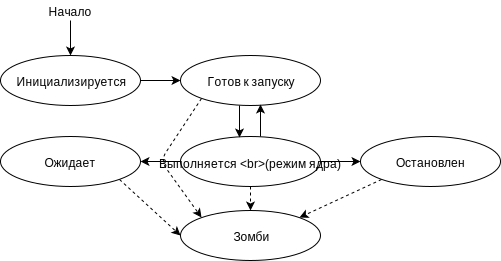
\includegraphics[width=0.7\textwidth]{./processes-and-threads/processes/lifecycle/proc-lifecycle.png}
\end{figure}

Когда инициализация процесса завершается --- он оказывается в стадии \textbf{“готов“}. С этого момента процесс находится в ожидании момента, когда его выберет планировщик процессов и даст ему какой-то квант процессорного времени.

При получении процессорного времени процесс переходит в состояние \textbf{“выполняется“}. Выполняться процесс может в режиме ядра --- при осуществлении системных вызовов, прерываний и в режиме задачи --- выполнять инструкции процессора. По окончании квоты времени, процесс может снова вернуться в состояние \textbf{“готов“}.

Также из состояния “выполняется“ процесс может перейти еще в два состояния --- \textbf{“остановлен“} и \textbf{“ожидает“}. Если он остановлен, то он остановлен пользователем (например, получен сигнал SIGSTOP). Ожидание наступает тогда, когда процессу нужны какие-то ресурсы. Как только условие, которого ждет процессор, выполняется, он переходит в состояние \textbf{“готов“}, то есть ожидает своей очереди на выполнение. 

Из каждого состояния процесс может перейти в в состояние \textbf{“зомби“}. Этот процесс нужен для того, чтобы родительский процесс мог получить код возврата этого процесса. Это промежуточное состояние --- процесса уже нет, но он технически еще есть. Тем не менее, это самое что ни на есть валидное состояние. 

\textbf{В какой момент процесс окончательно исчезает из таблицы процессов?}

После того как его родительский процесс вызовет wait (2), waitpid (2), waitid(2) - позволяет завершить процесс, если он таки стал зомби. 

Традиционная проблема --- порождая процесс, необходимо в какой-то момент сказать ему wait (2), чтобы не плодить зомби. В противном случае у вас может закончится лимит на создание новых процессов. 

\textbf{Что происходит с зомби, если его родитель не вызвал wait (2), а погиб?}

Его родителем становится init. Для всех процессов, которые становятся его потомками он делает wait (2). По факту, если вы написали какой-то код, который выполняет некоторое количество процессов после чего завершился, то на самом деле зомби в системе не останутся, т.к. после того как ваш основной процесс завершился, то потомков этого процесса подхватит init и он сам вызовет для них wait (2).

      \section{Создание процессов}

         \subsection{Семейство системных вызовов fork}
         Как мы помним, все процессы кроме init порождаются системными вызовами fork(2) или vfork(2). 

Системный вызов fork (2) создает дочерний процесс - точную копию родительского процесса. При успешном выполнении процессу родителю возвращается PID потомка, а потомку - 0.

\begin{CCode}{fork (2)}
	#include <sys/types.h>
	#include <unistd.h>
	
	pid_t fork(void); \end{CCode}

\begin{CCode}{Пример}
	int main(void) {
		pid_t pid;

		pid = fork(); /* change to vfork */
	
	    if (pid == 0) {
	        /* Now we're in child process */
		}   
		else {
			/* Now we're in parent process */
		}
		return EXIT_SUCCESS; 
	} \end{CCode}


Системный вызов vfork (2) определяется как fork (2) со следующим ограничением: поведение функции не определено, если созданный с её помощью процесс совершит хотя бы одно из следующих действий:

\begin{itemize}
	\item Произведет возврат из функции, в которой был вызван vfork (2);
	\item Вызовет любую функцию кроме \_exit() или exec* (2);
	\item Изменит любые данные кроме переменной, в которой хранится возвращаемое функцией vfork (2) значение.
\end{itemize}

\begin{CCode}{vfork (2)}
	#include <sys/types.h>
	#include <unistd.h>

	pid_t vfork(void); \end{CCode}

~\\~\\
\textbf{Разница между fork (2) и vfork (2).}

В отличие от fork (2), vfork (2) не создает копию родительского процесса, а создает разделяемое с родительским процессом адресное пространство до тех пор, пока не будет вызвана функция \_exit или одна из функций exec.
Родительский процесс на это время останавливает свое выполнение. Отсюда следуют и все ограничения на использование – дочерний процесс не может изменять никакие глобальные переменные или даже общие.

Другими словами, после вызова vfork() оба процесса будут видеть одни и те же данные и переменные.

Единственный вариант использования vfork --- когда вы предполагаете, что в скором будущем вы выполните функцию exec, которая заместит ваше адресное пространство новым исполняемым файлом. Соответственно, начиная с этого момента, будет разблокировано выполнение процесса родителя.

\begin{CCode}{Пример}
	int main(void) {
		pid_t pid;
		int status, common_var = 0;
	
		pid = fork(); /* change to vfork */
	
	    if (pid == 0) {
	        /* Child  */
			common_var = 1;
			printf("Child common_var value: %i \n",  common_var);
			
			exit(EXIT_SUCCESS);
		}   
		waitpid(pid, &status, 0);
		printf("Parent common_var value: %i \n",  common_var);
		
		if (common_var) {
			puts("vfork(): common variable has been changed");
		} else {
			puts("fork(): common variable hasn't been changed");
		}   
		return EXIT_SUCCESS; 
	} \end{CCode}

\begin{CCode}{Вывод для fork (2)}
	Child common_var value: 1 
	Parent common_var value: 0 
	fork(): common variable hasn't been changed \end{CCode}

\begin{CCode}{Вывод для vfork (2)}
	Child common_var value: 1 
	Parent common_var value: 1 
	vfork(): common variable has been changed \end{CCode}


         \subsection{Семейство системных вызовов exec}
         Мы уже сказали, что использование системного вызова vfork (2) рационально в случае дальнейшего запуска функции из семейства exec (3). Функция exec (3) загружает и запускает программу, заданную в аргументе path. Запущенная программа замещает адресное пространство текущего процесса. Все файлы вызывающей программы остаются открытыми и являются доступными новой программе.

Программа должна быть или двоичным исполняемым файлом, или скриптом, начинающимся со строки вида “#! интерпретатор [аргументы]“. 

\begin{CCode}{execle(3)}
	#include <unistd.h>

	int execle( 
		const char *path, 	/* path to file */ 
		const char *arg0, 	/* args */ /* ... */, 
		(char *)0,			/* NULL */ 
		char *const envp[] 	/* environment */ 
	); \end{CCode}

Семейство функций exec (По сути модификации execle)
	execlp() , execvp() , execl(), execv() , execle() , execve() 
		
Значения суффиксов l, v, p и e:

\begin{myenv}{p}{поиск программы по путям переменной окружения PATH. Без суффикса поиск будет производиться только в рабочем каталоге.}
\end{myenv}

\begin{myenv}{l}{показывает, что адресные указатели (arg0, arg1, ..., argn) передаются, как отдельные аргументы.}
\end{myenv}

\begin{myenv}{v}{показывает,  что  адресные  указатели  (arg[0], arg[1],...arg[n]) передаются, как массив указателей.}
\end{myenv}

\begin{myenv}{e}{показывает, что “дочернему“ процессу может быть передан  аргумент   envp (массив с переменными окружения).}
\end{myenv}


   \chapter{Межпроцессное взаимодействие}
   Далеко не всегда поставленную задачу можно решить используя только один процесс. В UNIX ОС существует некоторое количество механизмов для межпроцессного взаимодействия.

Перечислим их в произвольном порядке:

\begin{itemize}
	\item System V семафоры;
	\item каналы;
	\item сокеты;
	\item сигналы; 
	\item очереди сообщений; 
	\item System V разделяемая память;
	\item механизм STREAMS. 
\end{itemize}
	

      \section{Семафоры}
      \begin{defi}{Семафор}
	это объект синхронизации, имеющий множество состояний: 0(заблокирован), 1, 2, …, N
\end{defi}

Семафор представляет из себя счетчики, ограничивающий количество возможных одновременных пользователей ресурса. Значение семафора отражает количество свободных мест.

Семафоры находятся в адресном пространстве ядра, поскольку доступ к ним должны иметь все процессы.

\textbf{Примерный алгоритм работы с семафором}

Изначально семафору устанавливается целое положительное значение N --- максимальное значение одновременных пользователей какого-либо ресурса. 

Когда новый пользователь хочет захватить (начать работать с ресурсом), он уменьшает значение семафора на 1. Таким образом уже N-1 пользователей могут начать использовать ресурс в данный момент. После окончания работы с ресурсом, пользователь должен увеличить значение N на 1, тем самым освободив место для еще одного пользователя. 

Если значение N становится равным 0, это значит, что уже никто не может получить доступ к желаемому ресурсу.

Существуют POSIX и System V семафоры. Семафоры System V являются не отдельными счетчиками, а представляют из себя группу счетчиков, объединенных каким-либо признаком.

\begin{CCode}{Для работы с семафорами System V используются такие системные вызовы как:}
	#include <sys/sem.h>

	int semctl(int semid, int semnum, int cmd, ...);

	int semget(key_t key, int nsems, int semflg);

	int semids(int *buf, uint_t nids, uint_t *pnids);

	int semop(int semid, struct sembuf *sops, size_t nsops);

	int semtimedop(int semid, struct sembuf *sops, unsigned nsops,
			struct timespec *timeout); \end{CCode}

\begin{CCode}{Для работы с семафорами POSIX используются такие функции как:}
	#include <semaphore.h>

	int sem_wait(sem_t *sem);

	int sem_init(sem_t *sem, int pshared, unsigned int value);

	int sem_post(sem_t *sem);

	int sem_getvalue(sem_t *sem, int *sval);

	int sem_destroy(sem_t *sem); \end{CCode}

Вам предлагается ознакомиться с ними самостоятельно.

      \section{Каналы}

         \subsection{Неименованные каналы}
         Для создания неименованного калала существуют системные вызовы pipe (2) и pipe2 (2). Оба они принимают на вход массив из двух элементов. После успешного выполнения вызова массив содержит два файловых дескриптора: для чтения информации из канала и для записи в него соответственно. 

\begin{CCode}{pipe(2)}
	#include <unistd.h>
	
	int pipe(
		filedes[2]
	); \end{CCode}

Системный вызов pipe2 (2) принимает также некоторые флаги, влияющие на поведение канала.

Неименованные каналы можно использовать для родственных процессов. Когда процесс порождает другой процесс, дескрипторы родителя наследуются дочерним процессом, и, таким образом, осуществляется связь между двумя процессами. Один из них использует канал только для чтения, а другой только --- для записи.


         \subsection{Именованные каналы}
         Именованные каналы во многом работают так же, как и неименованные каналы, но все же имеют несколько заметных отличий.

\begin{itemize}
	\item именованные каналы существуют в виде специального файла устройства в файловой системе;
	\item процессы различного происхождения могут разделять данные через такой канал;
	\item именованный канал остается в файловой системе для дальнейшего использования и после того, как весь ввод/вывод сделан.
\end{itemize}


Существует два способа создания именованного канала:

Создать обычный файл, директорию или файл специального назначения с помощью системного вызова mknode (2), указав 0 в dev\_t.

\begin{CCode}{mknode (2)}
	int mknod(
		const char *path, 
		mode_t mode, 
		dev_t dev
	); \end{CCode}

или воспользоваться функцией mkfifo (3)

\begin{CCode}{mkfifo (3)}
	int mkfifo(
		const char *pathname, 
		mode_t mode
	); \end{CCode}
	

      \section{Сокеты}
      Как уже было сказано, сокеты --- это двусторонние каналы передачи данных между двумя единицами соединения. Существует несколько видов сокетов:

\begin{itemize}
	\item UNIX domain 
	\item Сетевые 
	\item BSD сокеты 
	\item Прочие
\end{itemize}

Они различаются по семействам адресов. 

Сокет подразумевает, что у вас есть некий сервер, который слушает определенный сокет.


\textbf{Для работы с сокетами существуют следующие системные вызовы.}

Cистемный вызов socket(2) создает новый сокет указанного типа и возвращает номер файлового дескриптора или код ошибки. В качестве аргументов этот системный вызов принимает семейство адресов, тип соединения и протокол.

\begin{CCode}{socket(2)}
	int socket( 
		int domain, 	/* address domain */ 
		int type,		/* type */ 
		int protocol	/* protocol (ex. tcp, udp) */ 
	); \end{CCode}

Системный вызов bind(2) используется на стороне сервера для того, чтобы ассоциировать сокет с адресом (описанным структурой address), например, адресом хоста и портом. Этот системный вызов возвращает 0 или код ошибки. Вызов принимает номер файлового дескриптора сокета, имя и длину поля имени.

\begin{CCode}{bind(2)}
	int bind( 
		int s, 							/* socket's descriptor number */ 
		const struct sockaddr *name, 	/* name */ 
		int namelen 					/* size of name in bytes */ 
	); \end{CCode}

Системный вызов listen(2) используется на стороне сервера для того, чтобы TCP сокет, связанный с адресом, начал “слушать” указанный порт. Системный вызов принимает номер файлового дескриптора сокета и длину очереди. Возвращает 0 или код ошибки.

\begin{CCode}{listen(2)}
	int listen( 
		int s, 			/* socket's descriptor number */ 
		int backlog 	/* length of queue */ 
	); \end{CCode}


Системный вызов accept(2) используется на стороне сервера. Принимает входящее соединение, создает новое TCP соединение и новый сокет, связанный с подключенным. Возвращает номер дескриптора или код ошибки.

\begin{CCode}{accept(2)}
	int accept( 
		int s, 					/* socket's descriptor number */ 
		struct sockaddr *addr,	/* client's address */ 
		socklen_t *addrlen 		/* size of client's address */ 
	); \end{CCode} 


Системный вызов connect(2) используется на стороне клиента и назначает свободный порт сокету. В случае TCP сокета пытается установить новое TCP соединение. Этот вызов принимает номер файлового дескриптора сокета, имя и длину поля имени. Он возвращает 0 или код ошибки.

\begin{CCode}{connect(2)}
	int connect( 
		int s,							/* socket's descriptor number */ 
		const struct sockaddr *name, 	/* name */ 
		int namelen 					/* size of name in bytes */ 
	); \end{CCode} 


      \section{Сигналы}
      \begin{defi}{Сигнал}
	механизм ОС для уведомления процесса о некотором событии. 
\end{defi}

Идея в том, что когда-то возникла необходимость асинхронно отправлять уведомления другому процессу о событии (как бы просто ставить галочку о том, что событие произошло). Для этой задачи и придумали механизм сигналов. 

В случае только межпроцессного взаимодействия ОС не гарантирует доставку сигналов. 

Есть определенное количество сигналов и, в зависимости от операционной системы, это количество меняется. Используя сигналы, нужно понимать, что это может сделать ваш код системно зависимым --- непереносимым.

Стандартных сигналов 16, но в большинстве ОС их немного больше. Они говорят о том, что нужно делать когда приходит сигнал такого типа. Вот некоторые из таких реакций:

\begin{myenv}{SIG\_IGN}{проигнорировать пришедший сигнал.} 
\end{myenv}

\begin{myenv}{SIG\_INT}{завершить процесс.} 
\end{myenv}
	
\begin{myenv}{SIG\_ERR}{завершить процесс с дампом памяти.}
\end{myenv}
	
\begin{myenv}{SIG\_HOLD}{позволяет остановить процесс.}
\end{myenv}

Существуют некоторые немаскируемые сигналы. В первую очередь, это сигнал \textbf{SIG\_KILL}. Дословно --- убить процесс. Однако, существует несколько случаев, при которых после вызова SIG\_KILL сигнал не будет убит сразу же:

\begin{itemize}
	\item когда процесс является зомби;

	\item когда процесс остановлен. Вы можете остановить выполнение процесса, но после того как вы его запустите он все же умрет;

	\item когда процесс находится в вызове системного вызова. До тех пор пока системный вызов не будет завершен сигнал не будет обработан
\end{itemize}

Легкий способ сделать неубиваемый процесс --- взять подключиться по сети к какой-нибудь файловой системе, открыть там файл и начать его читать, а потом физически выключить сервер. Вызов read (2) будет пытаться достучаться до сервера, который не будет отвечать. Убить такой процесс можно только двумя способами: включить сервер или перезагрузить систему. 

\begin{myenv}{SIG\_INT}{прерывание программы, которое обычно посылает эмулятор, поймавший обработку нажатия CTRL+C.}
\end{myenv}

Сигнал \textbf{SIG\_TERM} посылается, когда вы совершаете команду kill PID. Это еще один из тех сигналов, которые нельзя перехватить.

\begin{myenv}{SIG\_STOP}{останавливает процесс. Посылается после нажатия CTRL+Z всем процессам текущей группы. }

\begin{myenv}{SIG\_CONT}{продолжить выполнение, остановленного процесса}

\begin{myenv}{SIG\_ALARM}{вы можете воспользоваться этим сигналом в случае, если вы хотите уведомить сами себя через какое-то время, что ваше время истекло.}

\begin{myenv}{SIG\_PIPE}{вы можете получить данный сигнал, когда ваш сокет был неожиданно завершен второй стороной по какой-либо причине.}

\textbf{Сигналы SIG\_USR1 и SIG\_USR2} --- два стандартных сигнала, которые по умолчанию приводят к завершению процесса. Это такой способ послать уведомление процессу о том, что произошло что-то не предусмотренное стандартным поведением системы. 

         \subsection{Обработка сигналов}
         На все сигналы, кроме SIG\_STOP и SIG\_KILL, вы можете самостоятельно написать свой обработчик сигналов --- собственную функцию, которая будет реагировать на пришедший сигнал так, как вы в ней описали.

Свой обработчик сигналов можно сделать разными способами.

Библиотека libc предлагает механизм, который называется signal (3). Эта функция принимает в качестве аргементов номер сигнала и новую диспозицию сигнала. В качестве диспозиции можно подать функцию, которую вы хотите назначить обработчиком сигнала. Функция возвращает предыдущую диспозицию.

\begin{CCode}{signal (3)}
	#include <signal.h>

    void (*signal(int sig, void (*disp)(int)))(int); \end{CCode}
\\[0.5cm]

\textbf{Какие недостатки есть у signal (3)?}

Во многих реализация libC диспозиция сигнала устанавливается на действие по умолчанию каждый раз при получении сигнала.

Кроме того, у процесса в контексте есть такое понятие, как маска принимаемых сигналов. Фактически, это битовая последовательность, которая маскирует сигналы от принятия при их передаче. Если в этой битовой последовательности первый бит установлен в единицу, то, при попытке доставить сигнал процессу, операционная система увидит, что этот сигнал замаскирован, и поэтому его доставлять не нужно --- он будет просто отброшен.

Есть еще один более гибкий традиционно используемый способ обработки сигналов --- это системный вызов sigaction (2), который принимает числовой номер сигнала и два указателя на структуру sig\_action.

Первый указатель нужен для того, чтобы указать ОС, что мы хотим делать в случае прихода этого сигнала т.е. Во второй указатель помещается реакция на сигнал после выполнения системного вызова sigaction (2).

\begin{CCode}{sigaction (2)}
	#include <signal.h>

     int sigaction(int sig, const struct sigaction *restrict act,
         struct sigaction *restrict oact);  \end{CCode}

Структура sigaction включает в себя следующие поля:

\begin{itemize}
	\item void (*sa\_handler)(int) -- указатель на функцию обработчик сигнала;
	\item void (*sa\_sigaction)(int, siginfo\_t *, void *) -- указатель на функцию обработчик сигнала, если установлен флаг SA\_SIGINFO;
	\item sa\_flags -- флаги;
	\item sa\_mask -- битовая маска, которая маскирует прием/доставку сигналов процессу.
\end{itemize}
	

      \section{Очереди сообщений}
      \begin{defi}{Очередь сообщений}
	механизм передачи некоторого объема данных между процессами, основанный на сигналах
\end{defi}

Очередь сообщений используется, когда вам нужно передать какому-то клиенту или блоку информацию о том, что необходимо обработать. Позволяет передавать небольшие объемы данных между процессами. 

Очередь могут использовать все процессы, имеющие ключ и обладающие правами доступа к очереди (msg\_perm).

Структура сообщения очереди имеет следующие поля:

\begin{itemize}
	\item тип;
	\item длина сообщения в байтах;
	\item тело сообщения.
\end{itemize}

\begin{CCode}{Для реализации очередей используются такие системные вызовы как:}
	#include <sys/msg.h>

	int msgctl(int	msqid, int cmd,	struct msqid_ds	*buf);
	int msgget(key_t key, int msgflg);
	int msgsnd(int	msqid, const void *msgp, size_t	msgsz, int msgflg); \end{CCode}	

      \section{Разделяемая память}

      \section{Механизм STREAMS}
      Механизм STREAMS --- довольно устаревшая вещь. Альтернатива сокетам в System V.

Это модель, которая представляет собой поток, у которого есть некая вершина, набор драйверов и конечное устройство. 

Базовая единица STREAMS - stream, двунаправленный способ передачи данных между процессом в пользовательском пространстве и драйвером STREAMS в ядре. Stream состоит из заголовка, драйвера и N-го количество модулей.

\begin{figure}[htbp]
  \centering
  \includegraphics[width=0.15\textwidth]{./processes-and-threads/processes-interconnection/STREAMS/STREAMS.png}
\end{figure}

\textbf{Попробуем привести пример.}

Есть устройство, которое ничего не знает про TCP и UDP, оно знает MAC-адрес получателя и данные. Есть драйвер, который может запаковать IP-адрес в MAC-адрес и запаковать эти данные для сетевого устройства. Драйвер умеет только преобразовывать IP-адрес в MAC-адрес. 

Есть драйвер, который реализует работу с TCP и UDP, но ничего не знает про MAC-адреса, поэтому он подготавливает адреса для драйвера, который ниже. И так всё выше и выше, где есть вершина, которой мы говорим, что хотим отправить данные в таком-то направлении. 

Соответственно наши данные проходят через ряд настроенных нами драйверов. Эти драйвера оборачивают эти данные заголовками и отправляют в устройства. Устройства этот большой пакет отправляют в сеть. 

Модель красивая, потому что одна программа занимается ровно одной задачей. К сожалению, она несостоятельна, потому что постоянно копировать большие объемы данных внутри оперативной памяти даже быстрой всё равно медленно. Поэтому и не используется. 

STREAMS могут быть использованы для:

\begin{itemize}
	\item имплементации сетевых протоколов;
	\item разработки символьных устройств;
	\item разработки сетевых контроллеров (например, карты Ethernet);
	\item ввода-вывода на терминал.
\end{itemize}
	

   \chapter{Потоки}
   Какое есть недостаток у процессов? Для каждого процесса необходимо новое адресное пространство. Порождение процессов --- достаточно длительный и затратный процесс с точки зрения операционной системы. Альтернативой процессам являются потоки. Принципиальная разница в том, что они используют общее адресное пространство для нескольких наборов последовательно выполняемых команд.

\begin{defi}{Поток}
	наименьший набор инструкций, которым может быть выделена квота процессорного времени 
\end{defi}

Потоки одного процесса имеют единое с ним адресное пространство. Наиболее используемый стандарт –-- POSIX. Реализуются семейством функций с префиксом «pthread\_»

      \section{Легковесные процессы}
      \begin{defi}{Легковесный процесс}
	абстракция на уровне ядра ОС для описания процессов, разделяющих единое адресное пространство и системные ресурсы.
\end{defi}

      \section{Межпоточное взаимодействие}
      Для реализации межпоточного взаимодействия можно использовать:

\begin{itemize}
	\item Любое межпроцессное взаимодействие 
	\item mutex
	\item rwlock 
	\item volatile переменные 
	\item Общее адресное пространство
\end{itemize}

Отметим, однако, что не всякий вид межпроцессного взаимодействия разумно использовать для межпоточного взаимодействия.	

         \subsection{Общее адресное пространство}

         \subsection{Переменные volatile}
         Для межпоточного взаимодействия можно использовать глобальные переменные, помеченные ключевым словом volatile. Ключевое слово volatile инструктирует компилятор не оптимизировать доступ к переменной, а каждый раз использовать её значение из памяти.

C одной стороны, это замедляет работу, с другой --- гарантируется, что если кто-то другой изменил volatile-переменную, то вы прочитатете ее актуальное значение.		

         \subsection{Мьютексы}
         \begin{defi}{Мьютекс}
	простейший объект синхронизации, имеющий два состояния: «заблокирован» и «свободен».
\end{defi}

При использовании мьютекса только один поток в определенный момент времени может заблокировать мьютекс и получить доступ к разделяемому ресурсу. При завершении работы с ресурсом поток должен разблокировав мьютекс. 

Реализованы pthread\_mutex. 

\begin{CCode}{Приведем некоторые функции для работы с мьютексами:}
	#include <pthread.h>

	int pthread_mutex_init(pthread_mutex_t *mutex, 
            const pthread_mutexattr_t *attr);
	
	int pthread_mutex_destroy(pthread_mutex_t *mutex);

	int pthread_mutex_lock(pthread_mutex_t *mutex);

	int pthread_mutex_trylock(pthread_mutex_t *mutex);

	int pthread_mutex_unlock(pthread_mutex_t *mutex); \end{CCode}

Вам предлагается ознакомиться с ними самостоятельно.

Надо понимать, что используя мьютексы, вы можете эмулировать rwlock . Используя rwlock, вы можете эмулировать семафоры. Используя семафоры --- любое поведение. Самое главное --- вам нужно определиться, что и для какого случая использовать. Они условно взаимозаменяемы, но всё зависит от того, что конкретно вам нужно от кода.	

         \subsection{rwlock}
         Механизм rwlock --- чуть более продвинутая вещь, чем мьютекс. С rwlock вы можете не блокировать ресурс целиком, а, например, сделать его недоступным для записи, но доступным для чтения. 

\begin{CCode}{Механизм блокировок rwlock реализуется с помощью таких функций как:}
	#include <pthread.h>

    int pthread_rwlock_init(pthread_rwlock_t * restrict lock,
        const pthread_rwlockattr_t * restrict attr);

    int pthread_rwlock_destroy(pthread_rwlock_t *lock);

	int pthread_rwlock_wrlock(pthread_rwlock_t *lock);

    int pthread_rwlock_unlock(pthread_rwlock_t *lock); \end{CCode}	


\clearpage
\addcontentsline{toc}{chapter}{Литература}
\newpage

\begin{thebibliography}{99}

\bibitem{OSUNIX} Робачевский А. М., Немнюгин С. А., Стесик О. Л. Операционная система UNIX. — 2-еизд., перераб. и доп.— СПб.: БХВ-Петербург, 2008.

\bibitem{INSIDEUNIX} Вахалия Ю. UNIX изнутри — СПб.: Питер, 2003.
\end{thebibliography}

\end{document}
